\chapter{\texorpdfstring{\emph{The Margin That Shook the World}}{The Margin That Shook the World}}
\subsection{\texorpdfstring{\emph{How a Scribbled Note Launched Three Centuries of Mathematics --- and Why the Proof Would Never Have Fit}}{How a Scribbled Note Launched Three Centuries of Mathematics --- and Why the Proof Would Never Have Fit}}
\bigskip\noindent\rule{\linewidth}{0.4pt}\bigskip

\section{The Most Famous Scribble in History}
Here is a party trick that never fails to raise an eyebrow. Pick up a calculator --- or, if you are the sort of person who reads this book, a pencil --- and compute:

\[6^3 + 8^3 = 216 + 512 = 728.\]

Now compute \(9^3 = 729\). A miss --- by \emph{one}. The sum of two cubes, tantalizingly close to a perfect cube, misses by the slimmest of margins. Perhaps a bigger example will land? Try \(71^3 + 138^3 = 357{,}911 + 2{,}628{,}072 = 2{,}985{,}983\), and compare it with \(144^3 = 2{,}985{,}984\). Off by one again! It is as though the integers are playing a cosmic practical joke --- forever almost satisfying the equation, forever swerving away at the last instant.

The television show \emph{The Simpsons}, whose writing staff includes several mathematicians with a weakness for mischief, once flashed the equation

\[1782^{12} + 1841^{12} = 1922^{12}\]

on Homer's blackboard. Punch this into a pocket calculator and it checks out --- the left and right sides agree to ten digits. But it is false. The two sides differ by a number so large that it would take several lines to write down, yet so small \emph{relative} to the numbers involved that a na"ive calculator rounds them into agreement. Close only counts in horseshoes.


\begin{figure}[htbp]
\centering
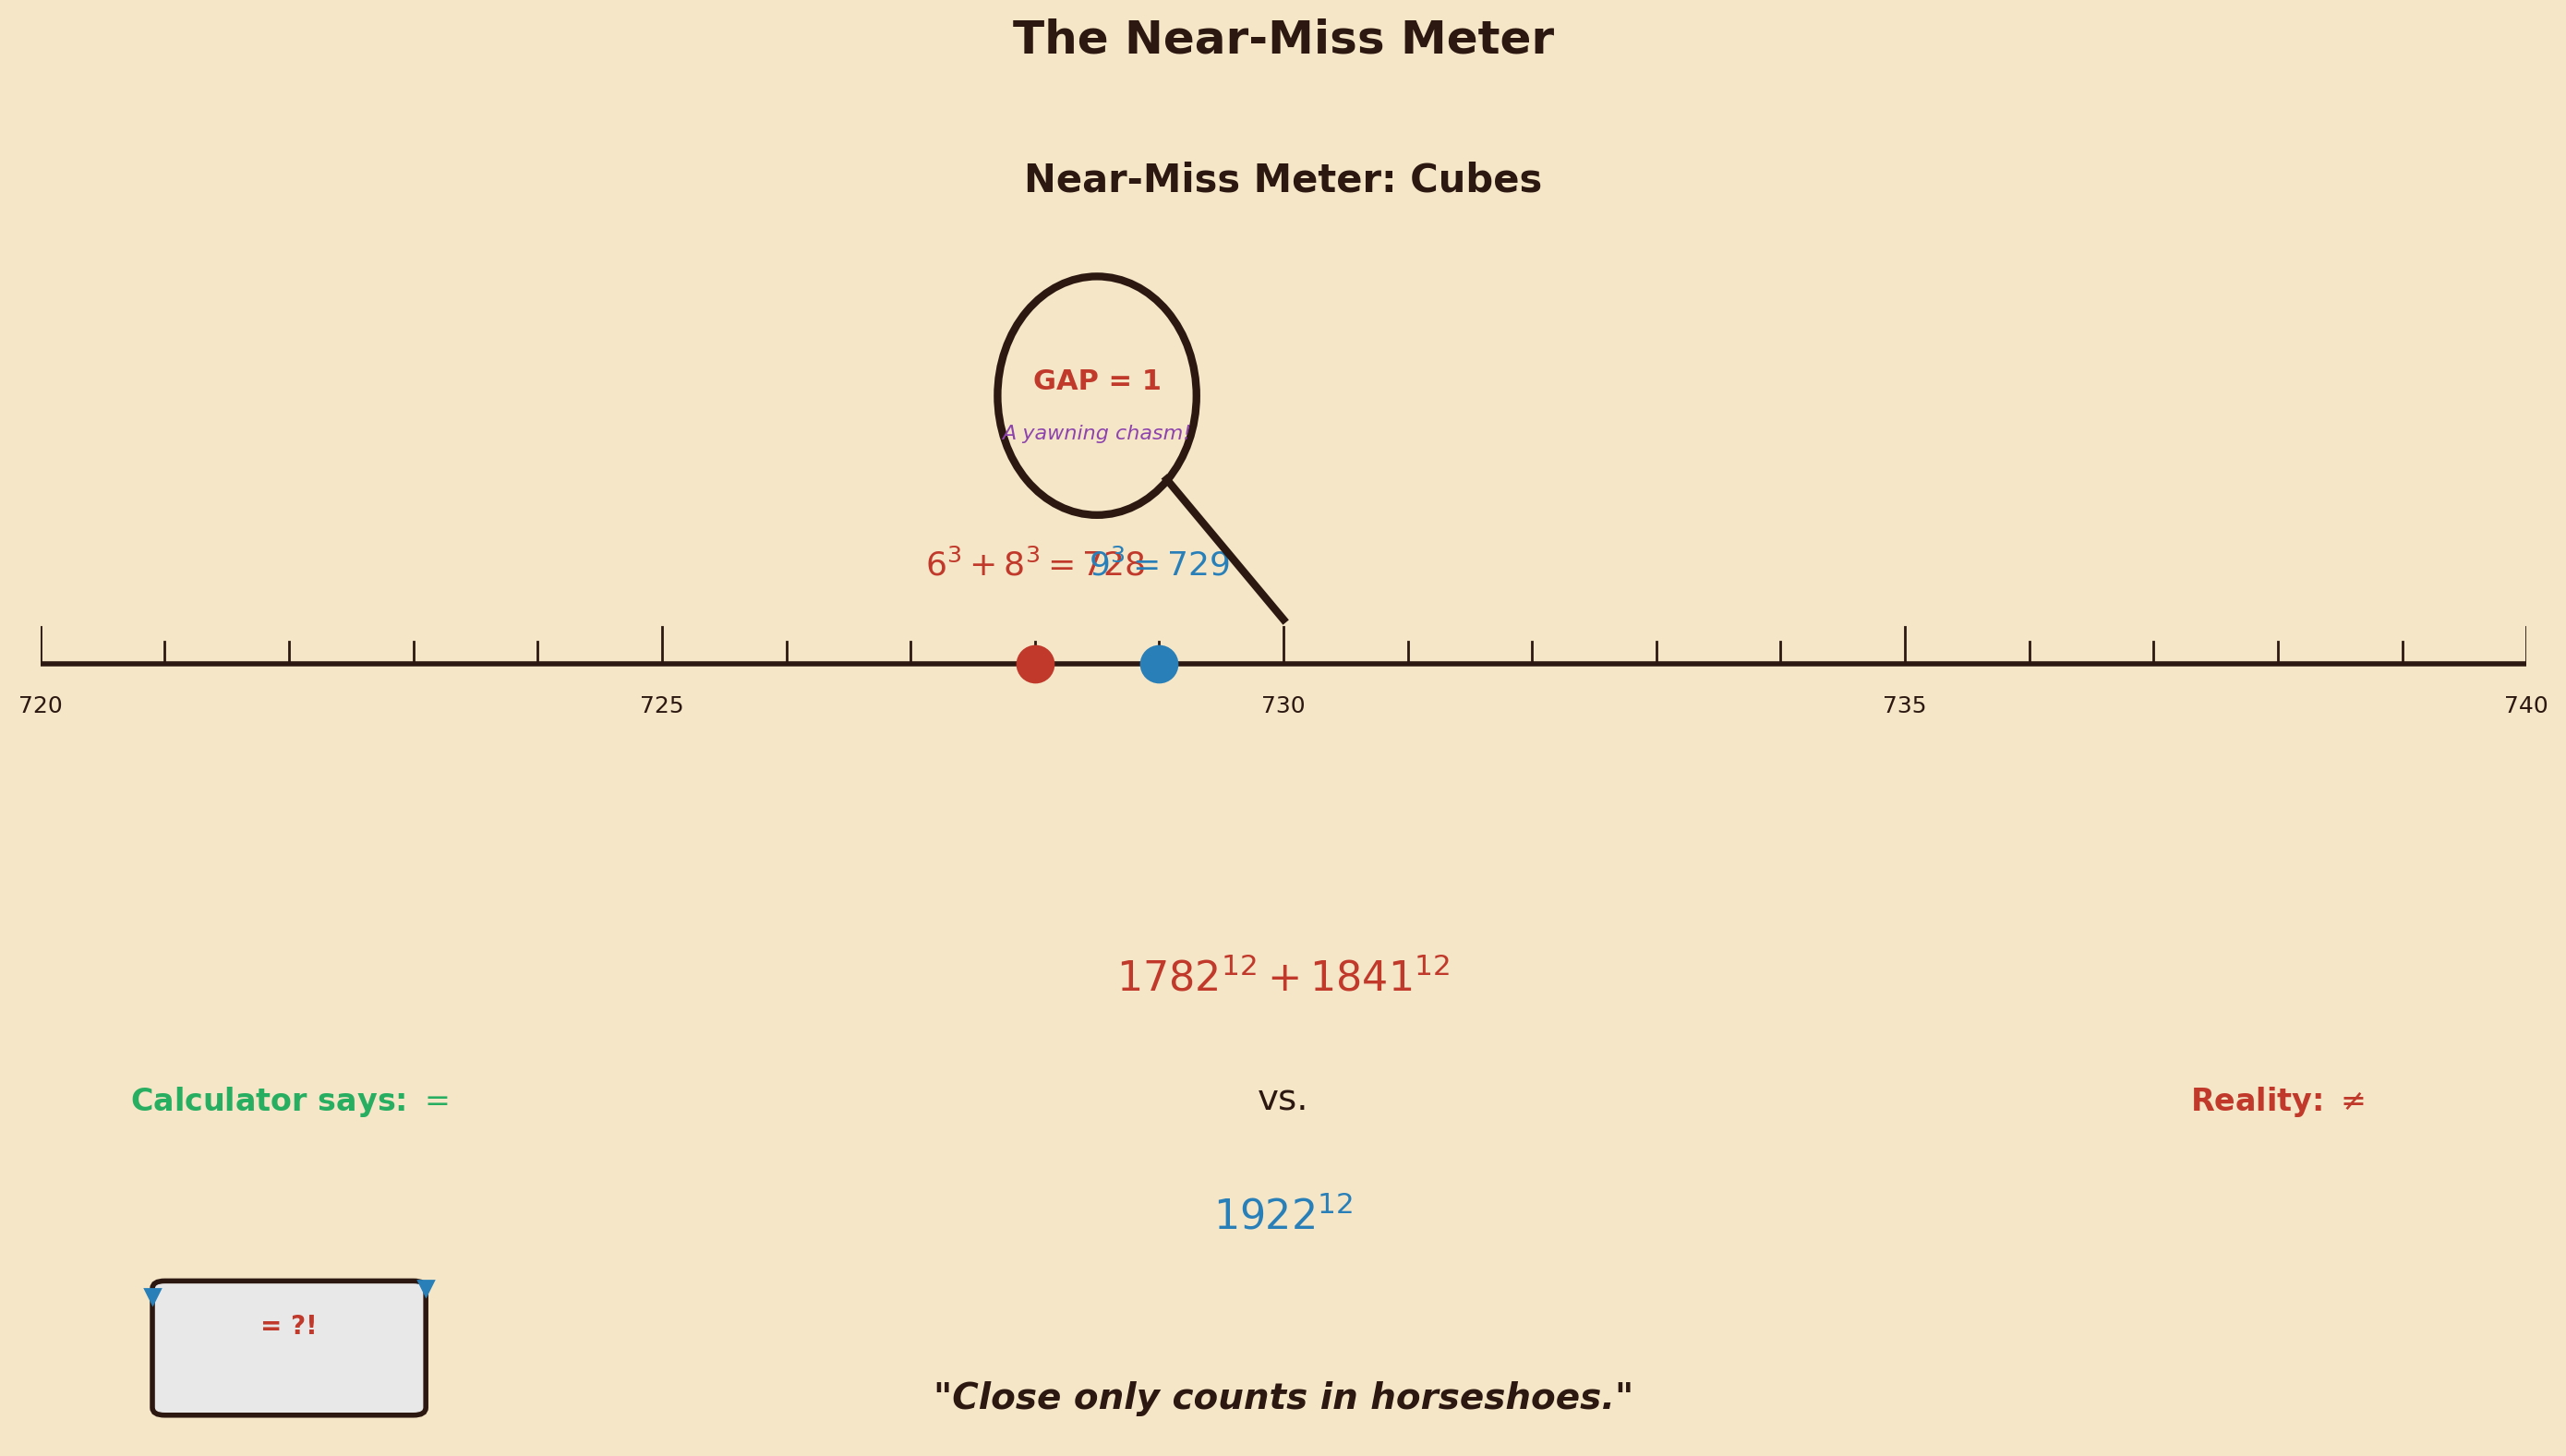
\includegraphics[width=0.85\textwidth]{Chapter10/images/fig01_near_miss_meter.png}
\caption{}
\end{figure}
A number line or ``near-miss meter'' showing how close \(6^3 + 8^3 = 728\) is to \(9^3 = 729\). A dramatic magnifying glass hovers over the gap of \(1\), enlarging it into a yawning chasm. A second row below shows the Simpsons equation \(1782^{12} + 1841^{12}\) versus \(1922^{12}\), with an even tinier relative gap but a large absolute one, captioned ``Close only counts in horseshoes.'' The style is whimsical, with a pocket calculator sweating nervously at the bottom.{]}

So here is the question that will occupy the rest of this chapter: \emph{Is it possible that, for every power beyond the square, these near-misses never quite land?}

The answer is yes, and the story of how we came to know it is the most dramatic tale in the history of mathematics. It begins with a marginal note.

In 1637, the French lawyer and amateur mathematician Pierre de Fermat was reading a Latin translation of the \emph{Arithmetica} of Diophantus, the great third-century algebraist of Alexandria. The particular passage concerned Pythagorean triples --- solutions to \(a^2 + b^2 = c^2\) --- and Fermat, scribbling in the narrow margin of the page, wrote words that would echo for 358 years:

\begin{quote}
\emph{Cubum autem in duos cubos, aut quadratoquadratum in duos quadratoquadratos, et generaliter nullam in infinitum ultra quadratum potestatem in duos eiusdem nominis fas est dividere. Cuius rei demonstrationem mirabilem sane detexi hanc marginis exiguitas non caperet.}
\end{quote}

In English: ``It is impossible to separate a cube into two cubes, or a fourth power into two fourth powers, or in general, any power higher than the second, into two like powers. I have discovered a truly marvelous proof of this, which this margin is too narrow to contain.''


\begin{figure}[htbp]
\centering
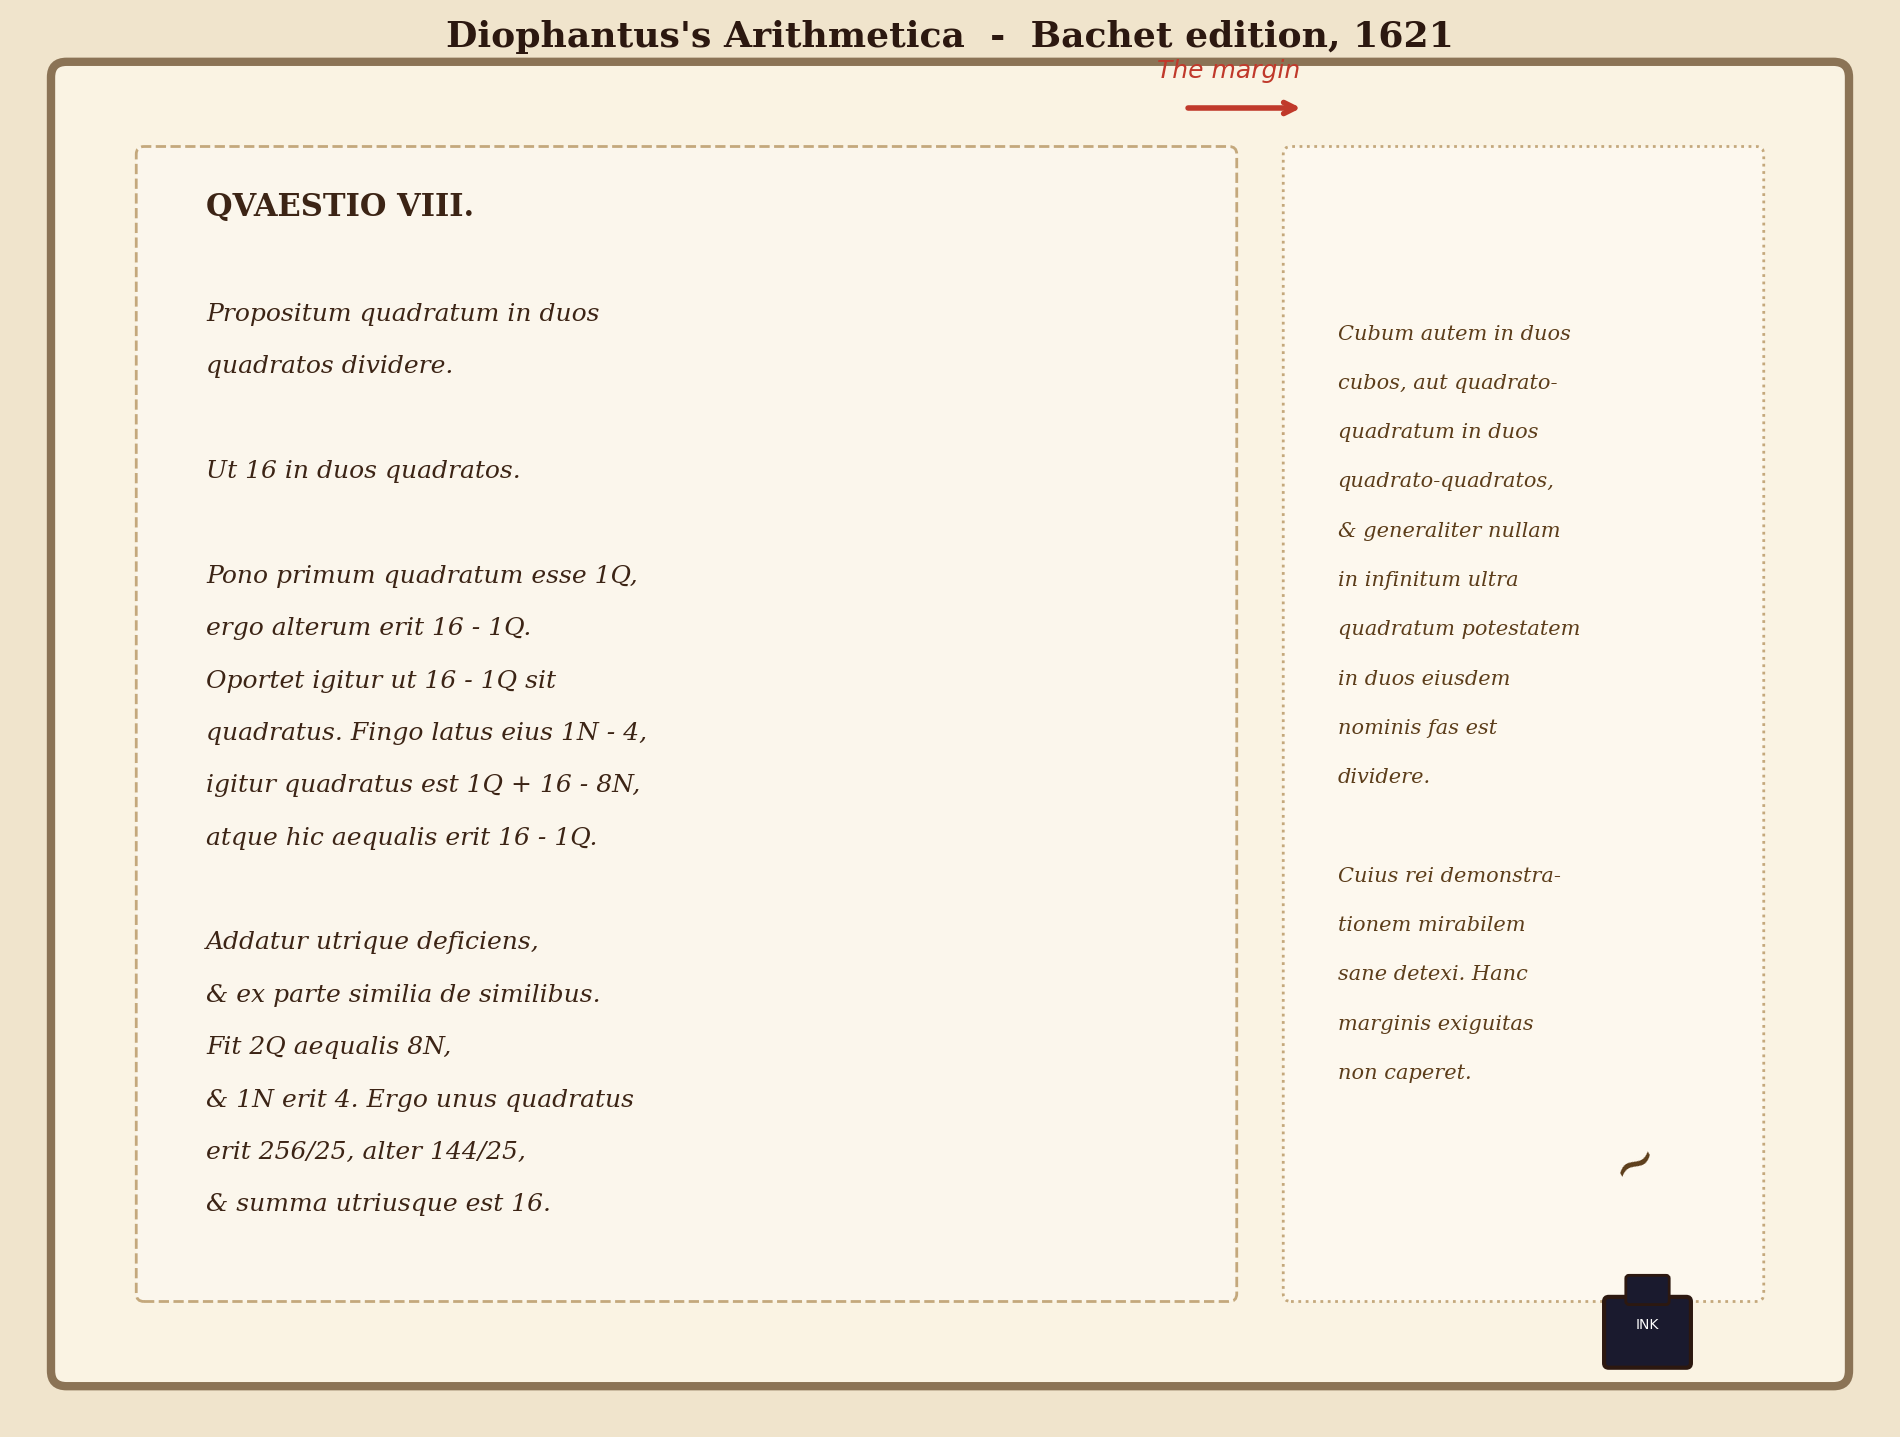
\includegraphics[width=0.85\textwidth]{Chapter10/images/fig02_fermat_margin.png}
\caption{}
\end{figure}
A facsimile-style rendering of a page from Diophantus's \emph{Arithmetica} (the 1621 Bachet edition), with Greek and Latin text in an elegant serif typeface. The right margin is visually, comically narrow --- barely two inches wide --- and contains Fermat's famous Latin annotation in a cramped 17th-century hand, with a small quill-pen flourish at the end. An ink bottle sits at the bottom corner, as though Fermat has just set down his pen.{]}

In modern notation, Fermat claimed:

\[\text{For every integer } n \ge 3, \text{ there are no positive integers } a, b, c \text{ with } a^n + b^n = c^n.\]

Or, in the compact language of quantifiers:

\[\forall\, n \ge 3,\; \forall\, a, b, c \in \mathbb{Z}^+, \quad a^n + b^n \neq c^n.\]

Contrast this with the case \(n = 2\). There, the Pythagorean triples pour forth in abundance. We met them in Chapter 1: \(3^2 + 4^2 = 5^2\), \(5^2 + 12^2 = 13^2\), \(8^2 + 15^2 = 17^2\), and infinitely many more. Every primitive triple arises from two parameters \(m > k > 0\) with \(\gcd(m, k) = 1\) and \(m \not\equiv k \pmod{2}\):

\[(a, b, c) = (m^2 - k^2,\; 2mk,\; m^2 + k^2).\]

An inexhaustible fountain of solutions. But the moment you raise the exponent from \(2\) to \(3\), the fountain dries up. Completely. Not a single solution survives. It is as though you have walked off a cliff --- one step separates infinite plenty from absolute nothing.

This is the theorem that became known as \textbf{Fermat's Last Theorem} --- ``last'' not because Fermat stated it last, but because it was the last of his many marginal claims to remain unproved. Every other assertion Fermat made was eventually verified or (occasionally) refuted. This one resisted for over three and a half centuries.

\bigskip\noindent\rule{\linewidth}{0.4pt}\bigskip

\section{The Art of Narrowing the Battle --- Reduction to Primes}
Before you storm a fortress, it helps to know which walls actually need storming.

Imagine a secret society of mathematicians --- the Order of the Exponent --- who divide the labor of proving Fermat's Last Theorem. Each member takes one exponent. Brother Anselm handles \(n = 3\). Sister Hypatia takes \(n = 4\). The enthusiastic novice volunteers for \(n = 6\). But a senior member taps the novice on the shoulder: ``Save your ink. If Anselm succeeds with \(n = 3\), you get \(n = 6\) for free.''

Why? Here is the trick. Suppose someone hands you a solution to \(a^6 + b^6 = c^6\). Write \(6 = 3 \times 2\). Then:

\[a^6 + b^6 = (a^2)^3 + (b^2)^3 = c^6 = (c^2)^3.\]

Set \(A = a^2\), \(B = b^2\), \(C = c^2\). These are positive integers, and \(A^3 + B^3 = C^3\). That is a solution to the \emph{cubic} Fermat equation --- which Brother Anselm has just proved impossible. Contradiction. No solution for \(n = 6\) exists.

The same domino trick works in general. If FLT holds for exponent \(n\), then it automatically holds for every multiple of \(n\):

\[a^{nk} + b^{nk} = c^{nk} \implies (a^k)^n + (b^k)^n = (c^k)^n,\]

and the right-hand side is a forbidden Fermat equation for exponent \(n\), with the positive-integer ``unknowns'' \(a^k\), \(b^k\), \(c^k\).

So which exponents must the Order actually tackle? Only the ones that are not multiples of smaller exponents --- the \emph{atoms} of the exponent world. A moment's reflection reveals:

\[n \ge 3 \implies 4 \mid n \;\text{ or }\; \exists\, p \ge 3 \text{ prime with } p \mid n.\]

Every integer \(n \ge 3\) is either a multiple of \(4\), or a multiple of some odd prime. (Some are both, but we only need one.) Therefore, it suffices to prove FLT for \(n = 4\) and for every odd prime \(p \ge 3\). Knock down those dominoes, and every composite exponent topples with them.


\begin{figure}[htbp]
\centering
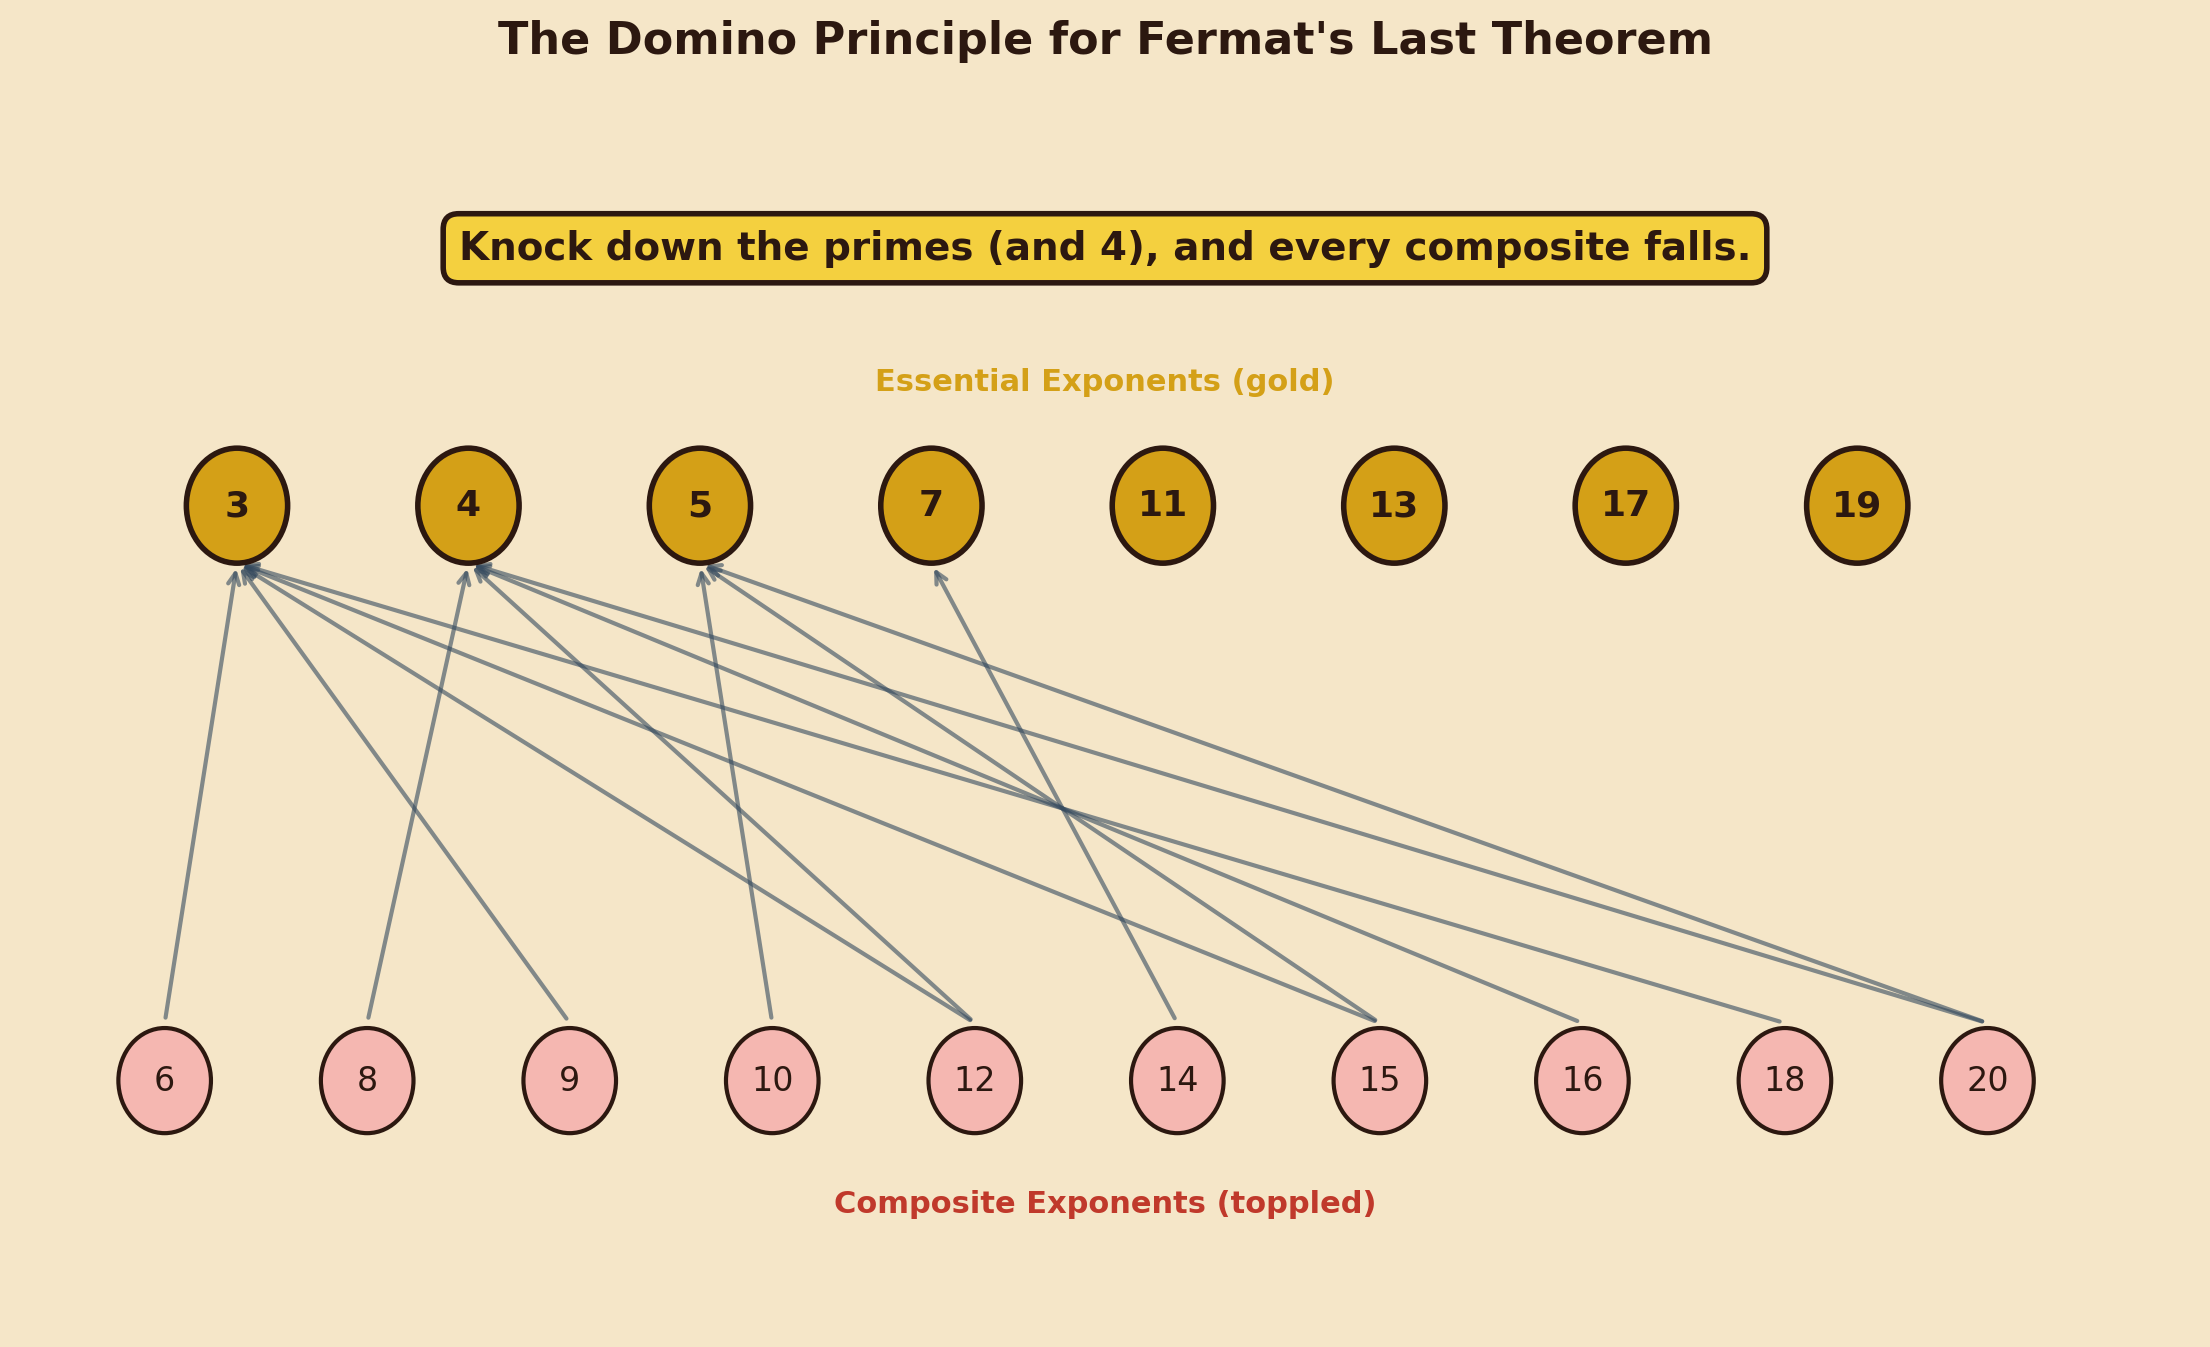
\includegraphics[width=0.85\textwidth]{Chapter10/images/fig03_factor_tree.png}
\caption{}
\end{figure}
A ``factor tree'' for the integers \(3\) through \(20\), arranged as a Hasse diagram. The nodes for \(4, 3, 5, 7, 11, 13, 17, 19\) are highlighted in gold as ``essential exponents.'' Each composite number (\(6, 8, 9, 10, 12, 14, 15, 16, 18, 20\)) has an arrow pointing down to the essential exponent that divides it. The visual metaphor is a row of dominoes: the golden essential exponents are standing upright at the back, and the composites are shown mid-topple in the foreground, cascading forward. A banner across the top reads: ``Knock down the primes (and \(4\)), and every composite falls.''{]}

This reduction was understood quite early --- certainly by Euler's time --- and is precisely why the cases \(n = 3\), \(n = 4\), \(n = 5\), \(n = 7\) received such intense individual attention throughout the eighteenth and nineteenth centuries. Each represented an irreducible fortress on the front line.

\bigskip\noindent\rule{\linewidth}{0.4pt}\bigskip

\section{\texorpdfstring{Fermat's Own Triumph --- The Case \(n = 4\)}{Fermat's Own Triumph --- The Case n = 4}}
Let us play a game. Take any right triangle with whole-number sides --- any Pythagorean triple --- and compute its area. The triple \((3, 4, 5)\) gives area \(\tfrac{1}{2} \cdot 3 \cdot 4 = 6\). Not a perfect square. Try \((5, 12, 13)\): area \(30\). Not a square. Try \((8, 15, 17)\): area \(60\). Try \((20, 21, 29)\): area \(210\). Try as many as you like --- I will wait. You will never find a right triangle with integer sides whose area is a perfect square. Never.

This is not a coincidence. It is a theorem. And it is secretly equivalent to Fermat's Last Theorem for the exponent \(n = 4\).

The method of proof is the one technique Fermat described explicitly, and it is among the most beautiful ideas in all of number theory: \textbf{infinite descent}. The strategy is elegant in its brutality. You assume a minimal solution exists --- one with the smallest possible value of \(c\). From this minimal solution, you extract, by a chain of algebraic manipulations and Pythagorean parametrizations, a strictly \emph{smaller} solution. But this contradicts the assumption of minimality. The original solution cannot exist.

Picture an infinite staircase, each step lower than the last, descending through the positive integers:

\[c_1 > c_2 > c_3 > \cdots > 0, \quad c_i \in \mathbb{Z}^+.\]

Such a sequence is impossible --- the positive integers have a floor. You cannot descend forever. And so the hypothetical solution, which set the staircase in motion, could never have existed in the first place.


\begin{figure}[htbp]
\centering
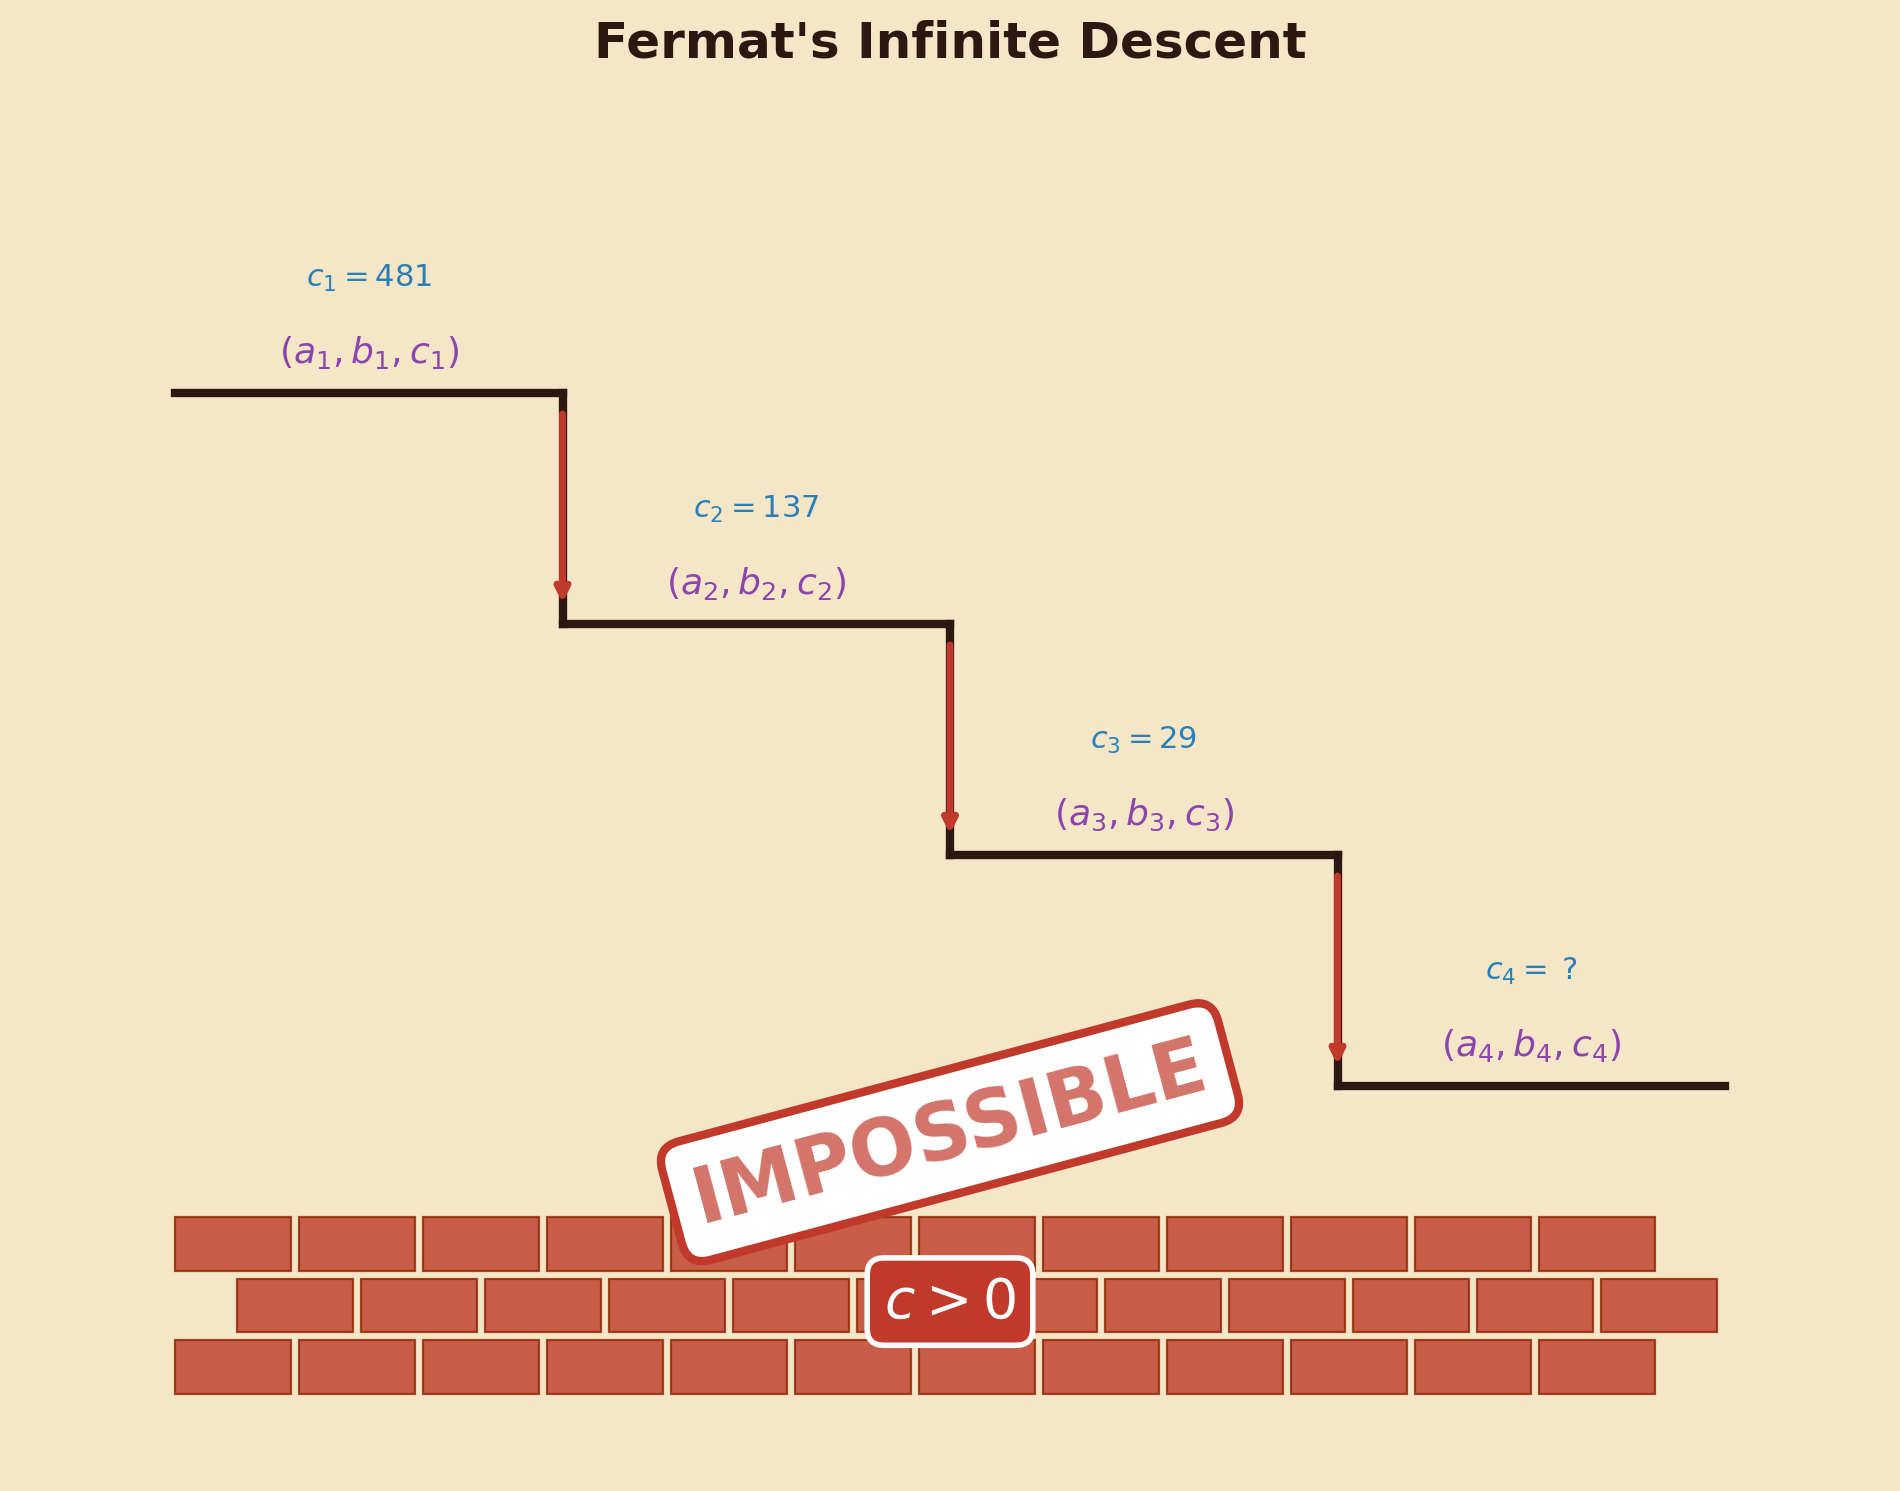
\includegraphics[width=0.85\textwidth]{Chapter10/images/fig04_descent_staircase.png}
\caption{}
\end{figure}
An Escher-inspired infinite staircase descending through the positive integers. Each step is labeled with a ``solution'' \((a_i, b_i, c_i)\), with \(c_i\) visibly decreasing: \(c_1 = 481\), \(c_2 = 137\), \(c_3 = 29\), \(c_4 = ?\). The staircase terminates at a brick wall labeled ``\(c > 0\)'' stamped with a large red ``IMPOSSIBLE.'' The perspective is slightly vertiginous, drawn in the style of M. C. Escher's impossible architectures, conveying the logical inevitability of the contradiction.{]}

Fermat's descent for \(n = 4\) works roughly as follows. A hypothetical solution \(a^4 + b^4 = c^4\) can be rewritten as \((a^2)^2 + (b^2)^2 = (c^2)^2\), a Pythagorean triple in disguise. Apply the parametric formula for Pythagorean triples to express \(a^2\), \(b^2\), and \(c^2\) in terms of two parameters. This reveals new arithmetic relationships among the parameters --- relationships that, when you tug on them hard enough, unravel into \emph{another} equation of the same form, but with a smaller hypotenuse. Pull again, and a still smaller equation falls out. The staircase descends, the floor rises up, and the whole structure collapses into contradiction.


\begin{figure}[htbp]
\centering
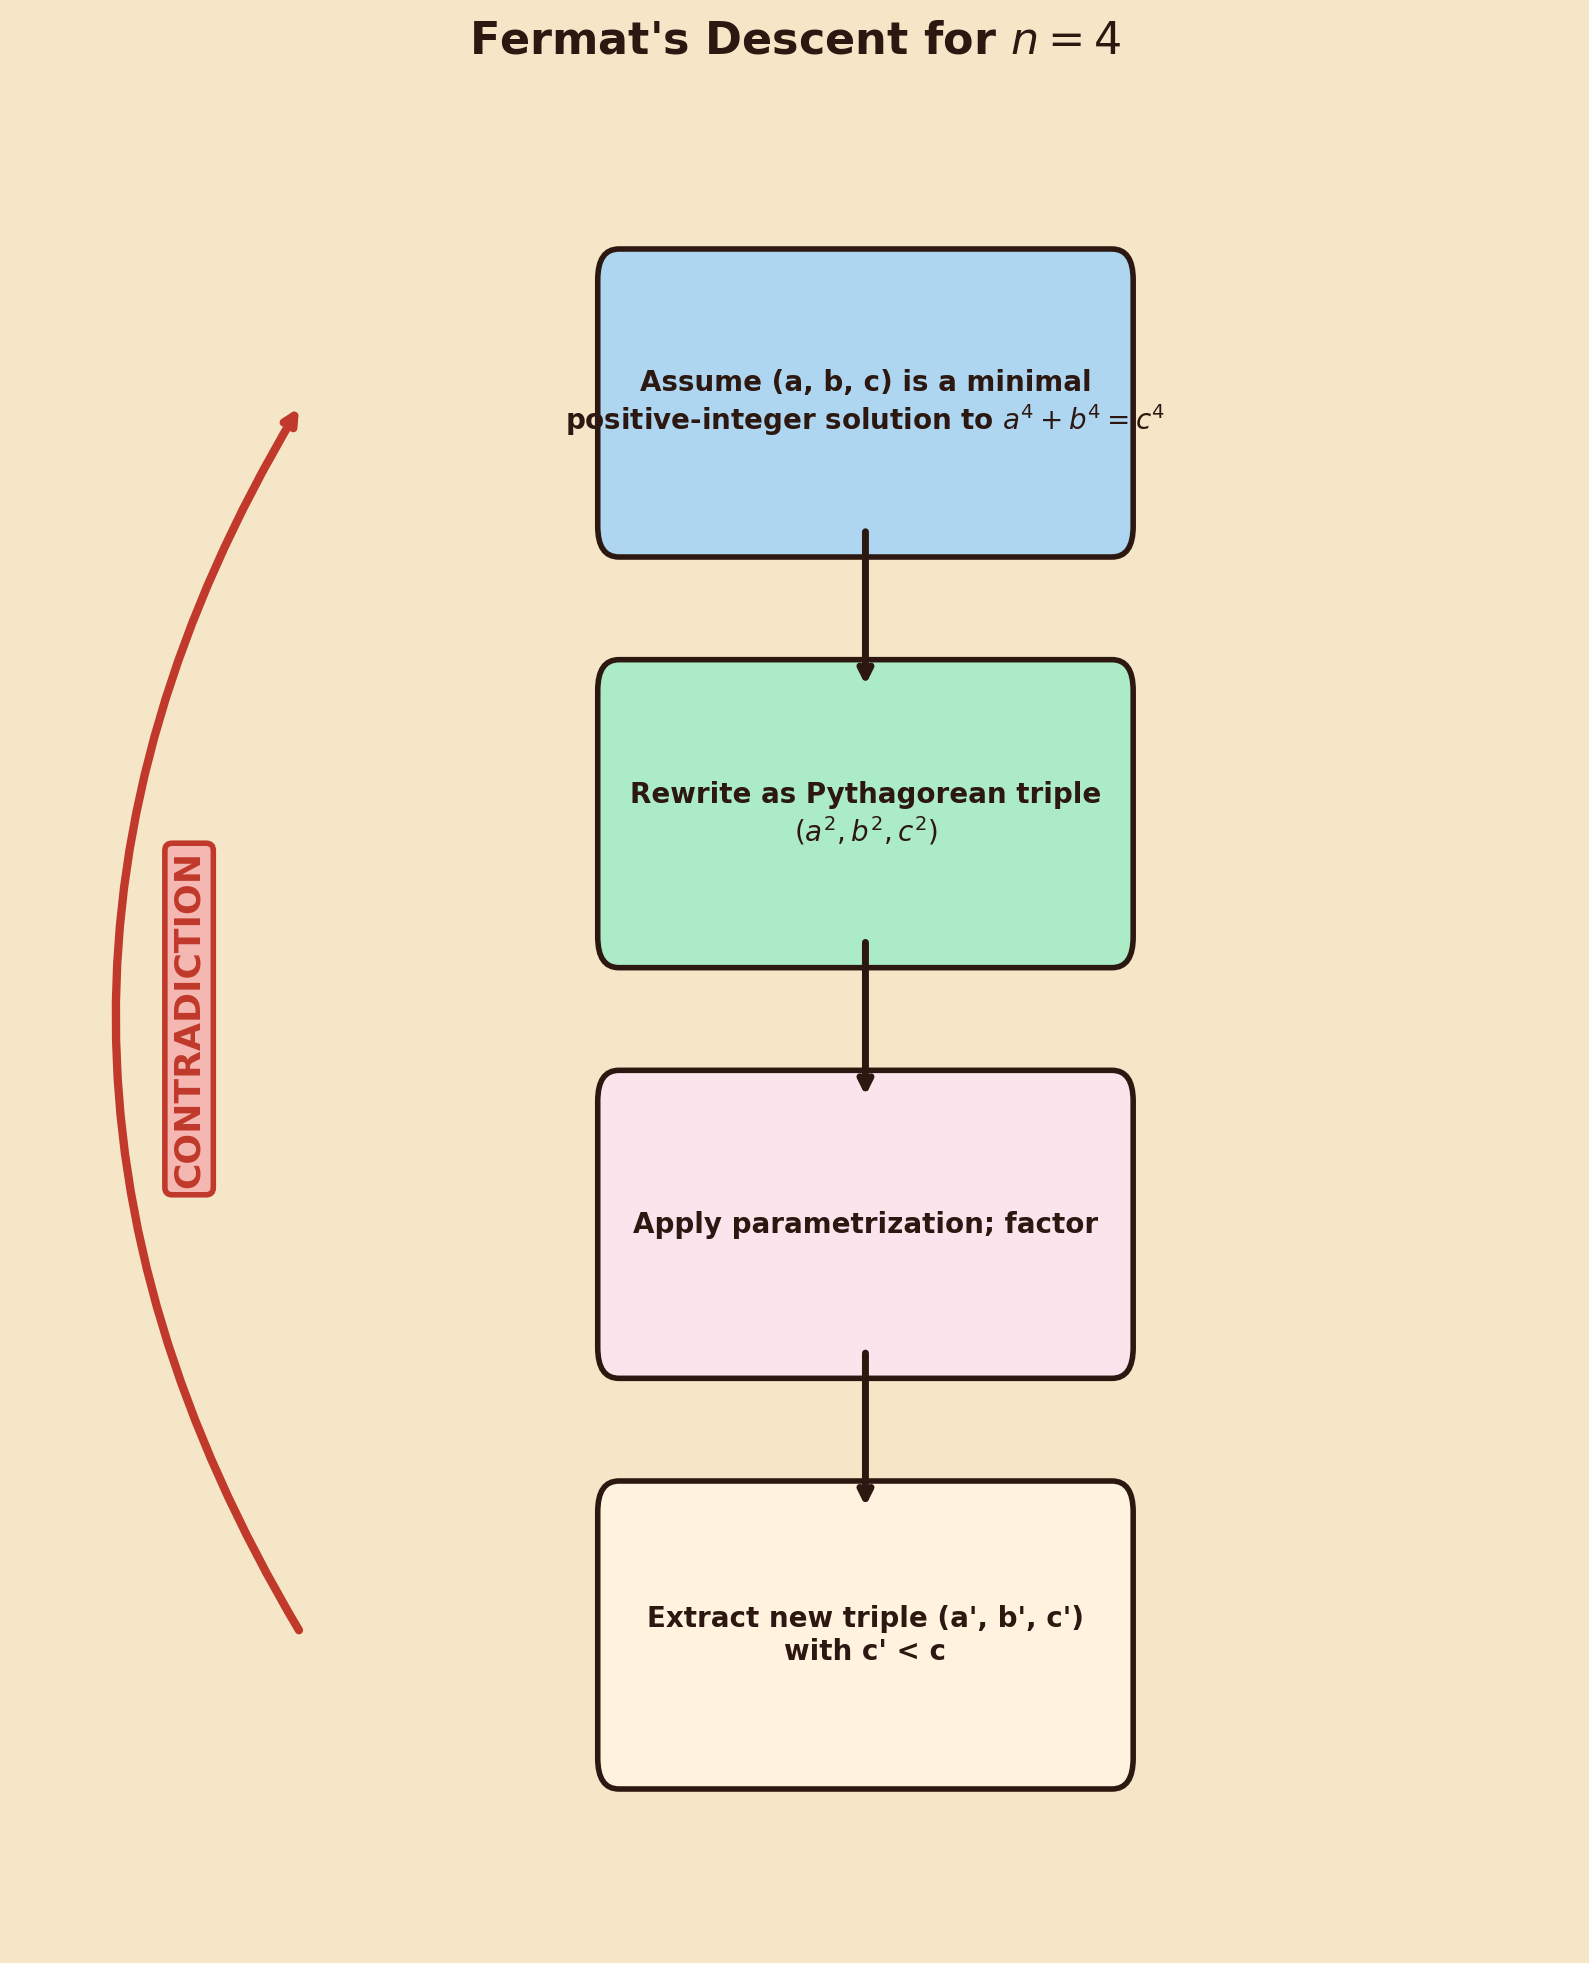
\includegraphics[width=0.85\textwidth]{Chapter10/images/fig05_descent_flowchart.png}
\caption{}
\end{figure}
A flowchart showing the descent argument for \(n = 4\). A box at the top reads ``Assume \((a, b, c)\) is a minimal positive-integer solution to \(a^4 + b^4 = c^4\).'' An arrow leads to ``Rewrite as Pythagorean triple \((a^2, b^2, c^2)\).'' Another arrow leads to ``Apply parametrization; factor.'' Another arrow leads to ``Extract new triple \((a', b', c')\) with \(c' < c\).'' A red arrow loops back to the top with a large ``CONTRADICTION'' label. The flowchart is clean and readable, with each box lightly shaded in a different pastel color.{]}

Infinite descent anticipates the well-ordering principle --- the axiom that every nonempty set of positive integers has a least element --- and is a forerunner of mathematical induction run backwards. Where induction climbs from \(1\) to \(2\) to \(3\) and beyond, descent plunges from \(n\) to \(n - 1\) to \(n - 2\), demonstrating that certain properties \emph{cannot} hold anywhere, because holding anywhere would force them to hold everywhere below, which is absurd. It is induction's dark twin, and one of the most powerful weapons in the number theorist's arsenal.

\bigskip\noindent\rule{\linewidth}{0.4pt}\bigskip

\section{The Stronger Weapon --- Why Squares Are Harder Than Fourth Powers}
Here is a subtle point that rewards careful attention. Fermat did not merely prove that \(a^4 + b^4 = c^4\) has no solutions. He proved something \emph{stronger}:

\[\text{There are no positive integers } a, b, c \text{ with } a^4 + b^4 = c^2.\]

Read that again. The right-hand side is \(c^2\), not \(c^4\). Since \(c^4 = (c^2)^2\) is a \emph{special case} of a perfect square, ruling out all squares on the right side is a more sweeping prohibition. If even \(c^2\) is too much to hope for, then \(c^4\) --- which demands that \(c^2\) itself be a perfect square --- is certainly out of reach. The stronger theorem implies the weaker one immediately:

\[a^4 + b^4 \neq c^2 \;\;\Longrightarrow\;\; a^4 + b^4 \neq (c^2)^2 = c^4.\]


\begin{figure}[htbp]
\centering
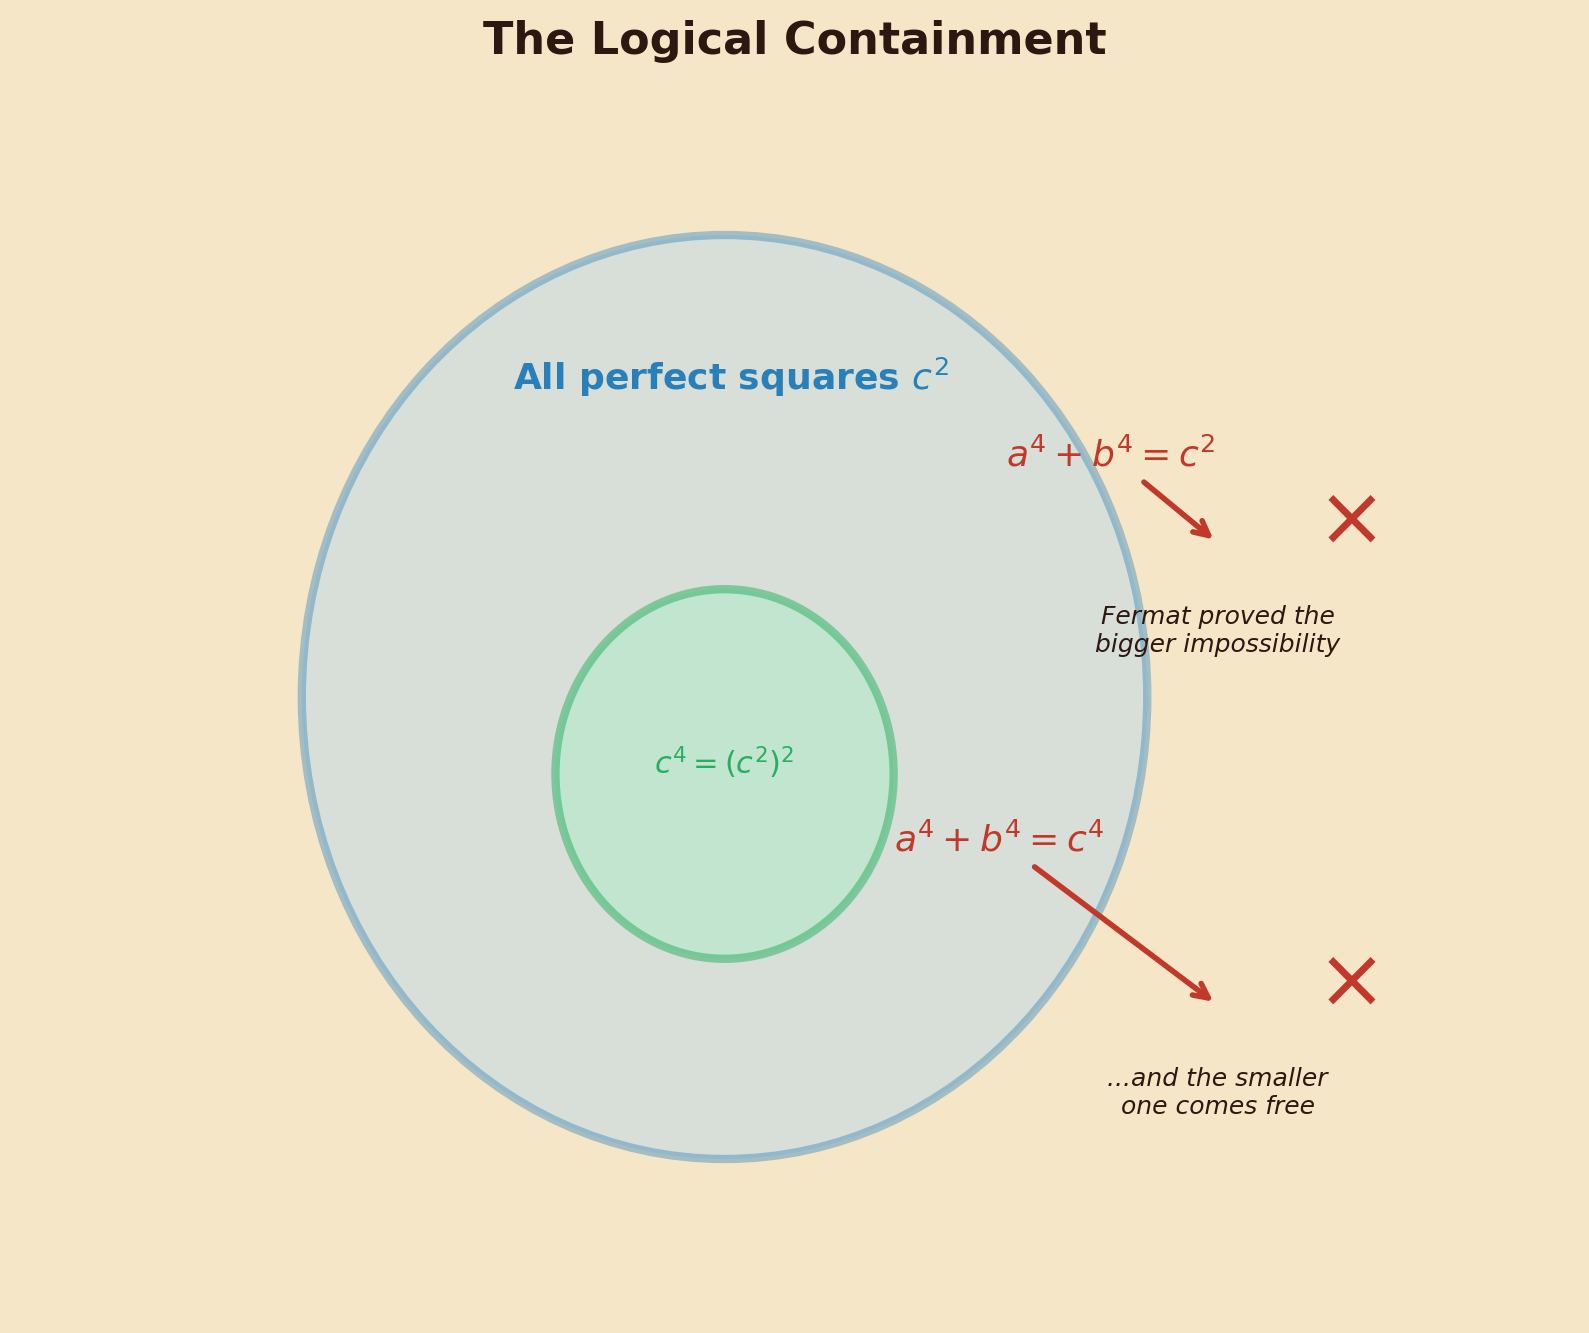
\includegraphics[width=0.85\textwidth]{Chapter10/images/fig06_venn_diagram.png}
\caption{}
\end{figure}
A Venn-diagram-style picture. The outer circle, drawn large, is labeled ``all perfect squares \(c^2\).'' Nested inside it, a much smaller circle is labeled ``perfect fourth powers \(c^4 = (c^2)^2\).'' A bold arrow from the outer circle to the equation \(a^4 + b^4 = c^2\) is crossed out with a red \(\times\), captioned ``Fermat proved the bigger impossibility.'' A thinner arrow from the inner circle to \(a^4 + b^4 = c^4\) is also crossed out, captioned ``\ldots and the smaller one comes free.'' The visual makes the logical containment immediately intuitive.{]}

Why bother with the stronger statement? Because it is mathematically equivalent to the assertion that no right triangle with integer sides has an area that is a perfect square --- the very puzzle we opened with. The proof of the stronger claim is what Fermat actually communicated, and it is one of the few complete proofs he ever wrote down. The descent is more intricate than for the weaker statement alone, but the payoff is richer: you get two theorems for the price of one.

\bigskip\noindent\rule{\linewidth}{0.4pt}\bigskip

\section{\texorpdfstring{Euler and the Cube --- The Case \(n = 3\)}{Euler and the Cube --- The Case n = 3}}
Every story about number theory eventually arrives at the doorstep of Leonhard Euler, and this one is no exception. In 1769, Euler ventured a bold generalization of Fermat's claim: he conjectured that it takes at least \(n\) many \(n\)-th powers to sum to an \(n\)-th power. Fourth powers require at least four summands; fifth powers require at least five; and so on. The conjecture stood, unquestioned, for nearly two centuries --- until 1966, when L. J. Lander and T. R. Parkin fed a computer and discovered:

\[27^5 + 84^5 + 110^5 + 133^5 = 144^5.\]

Only four fifth powers, not five. Euler's generalization was dead. But the sweet irony is that Euler himself had been right about the base case: the cube. In 1770, Euler published a proof that

\[\text{there are no positive integers } a, b, c \text{ with } a^3 + b^3 = c^3.\]

His strategy was revolutionary. Instead of working in the ordinary integers, he left \(\mathbb{Z}\) behind entirely and entered a new number system --- the \textbf{Eisenstein integers}, \(\mathbb{Z}[\omega]\), where \(\omega = e^{2\pi i / 3}\) is a primitive cube root of unity:

\[\omega = \frac{-1 + \sqrt{-3}}{2}, \qquad \omega^2 + \omega + 1 = 0, \qquad \omega^3 = 1.\]

In this system, every integer of the form \(a + b\omega\) (with \(a, b \in \mathbb{Z}\)) is an ``Eisenstein integer,'' and the ordinary laws of arithmetic --- addition, multiplication, divisibility --- extend naturally. The crucial advantage is that \(a^3 + b^3\) factors beautifully:

\[a^3 + b^3 = (a + b)(a + \omega b)(a + \omega^2 b) = c^3.\]

Three factors on the left, a perfect cube on the right. If these three factors are pairwise coprime (which can be arranged after dividing out common factors), and if the Eisenstein integers enjoy \emph{unique factorization}, then each factor must individually be a cube --- up to units --- and one can apply a descent argument to derive a contradiction.


\begin{figure}[htbp]
\centering
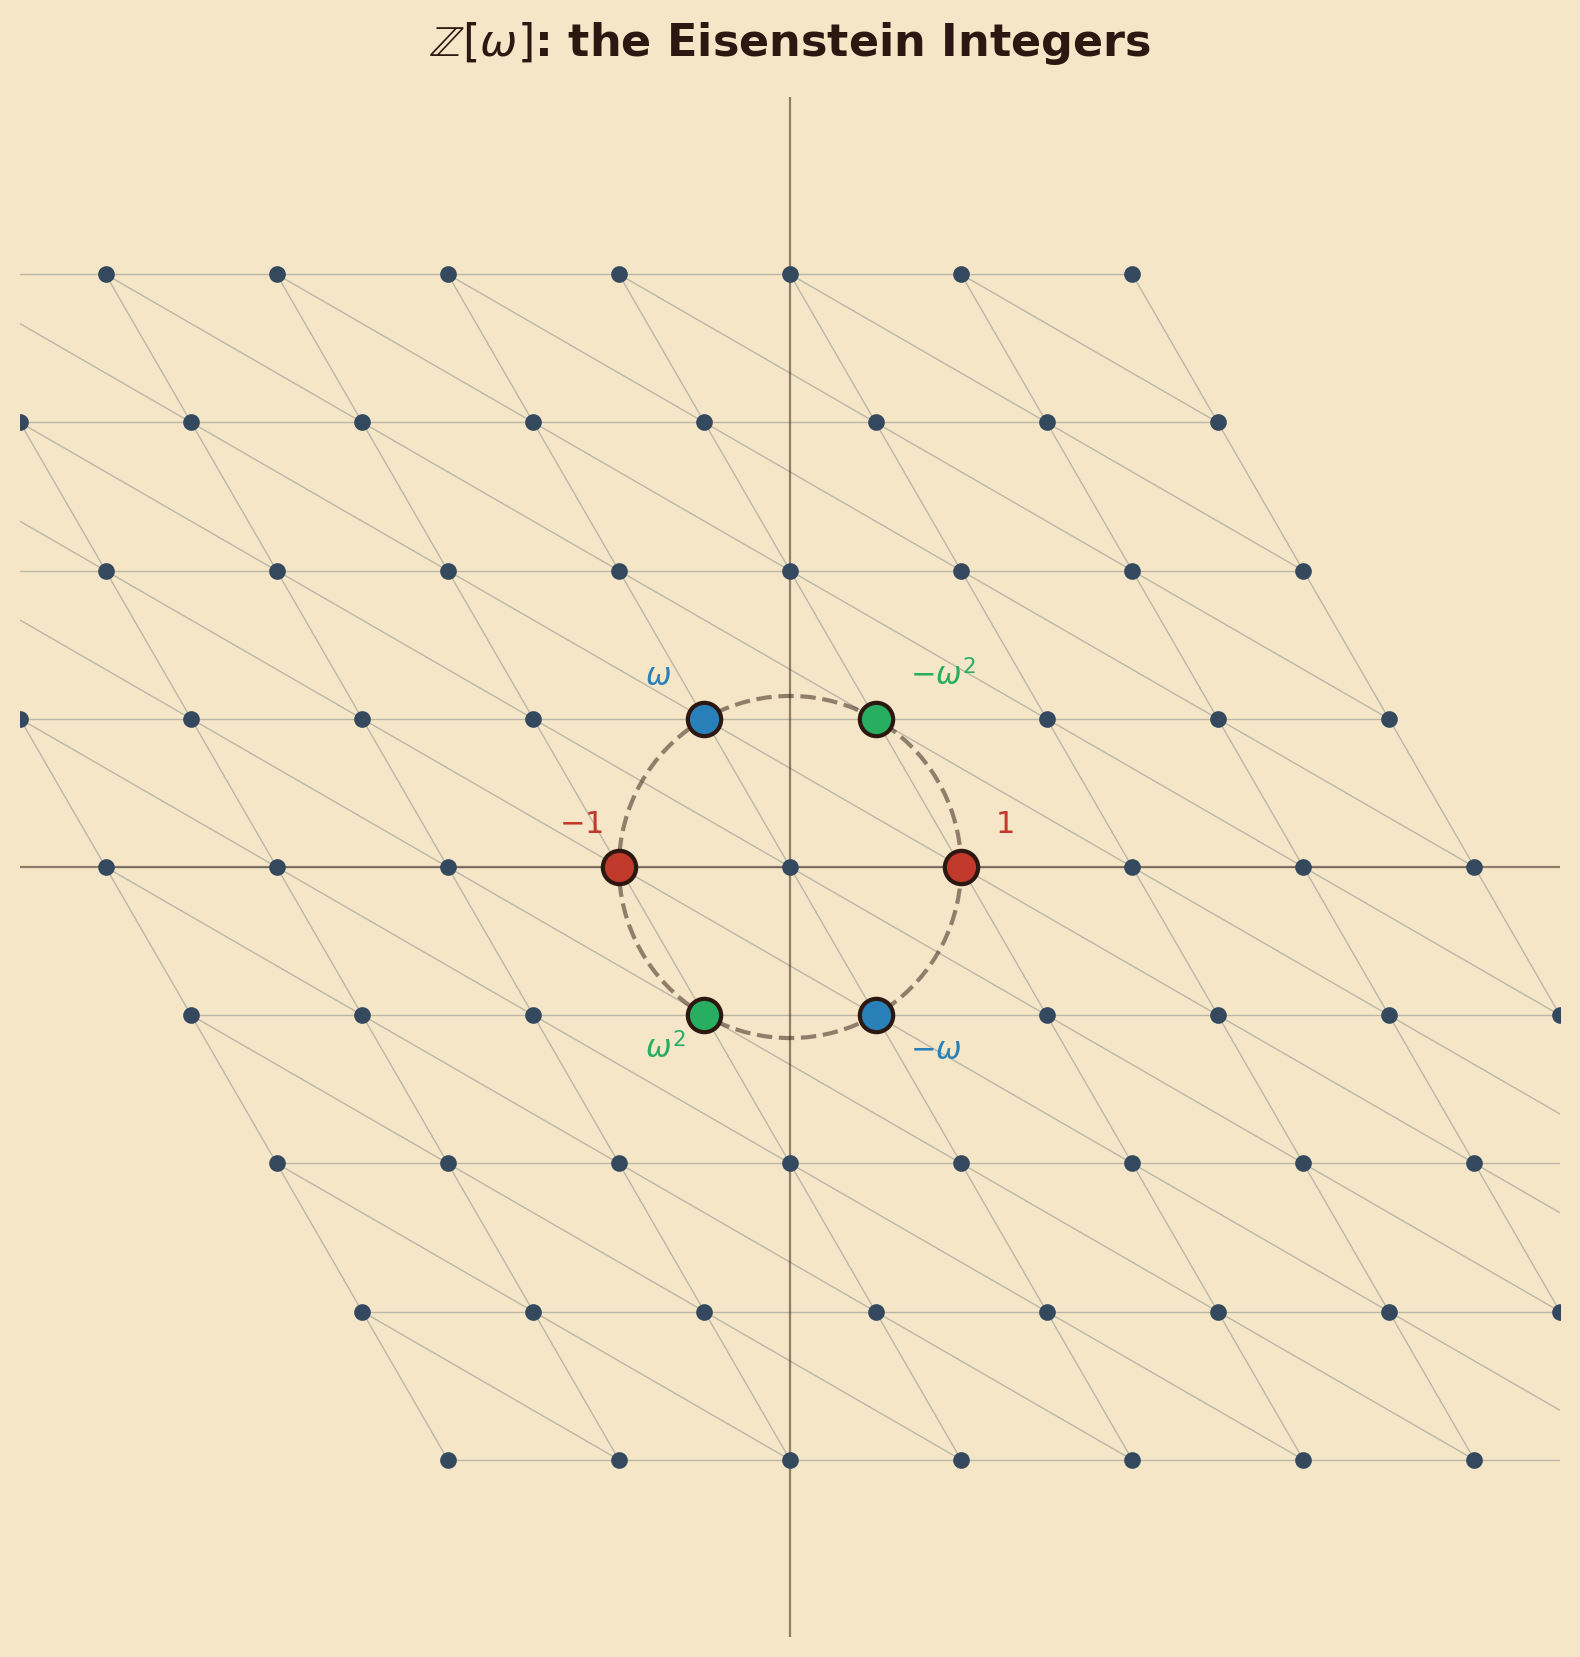
\includegraphics[width=0.85\textwidth]{Chapter10/images/fig07_eisenstein_lattice.png}
\caption{}
\end{figure}
The Eisenstein integers as a triangular lattice in the complex plane. Points are plotted at all values \(a + b\omega\) for integers \(a, b\) with \(|a|, |b| \le 4\). The lattice has a striking hexagonal symmetry. The unit circle is drawn as a dashed circle, and the six units \(\pm 1, \pm \omega, \pm \omega^2\) are highlighted as large colored dots on the circle. Faint lines connect nearest-neighbor lattice points, revealing the equilateral-triangle tiling. A label at the top reads ``\(\mathbb{Z}[\omega]\): the Eisenstein integers.''{]}

There is a gap in Euler's proof --- or rather, an assumption he made without checking. He took for granted that \(\mathbb{Z}[\omega]\) has unique factorization. Fortunately, it does: the Eisenstein integers form what algebraists call a \emph{principal ideal domain}, and unique factorization is guaranteed. But Euler did not prove this; he merely used it. The gap was filled by later mathematicians, and the proof stands correct. Euler's instinct was, as so often, unerring --- even when his rigor was not.


\begin{figure}[htbp]
\centering
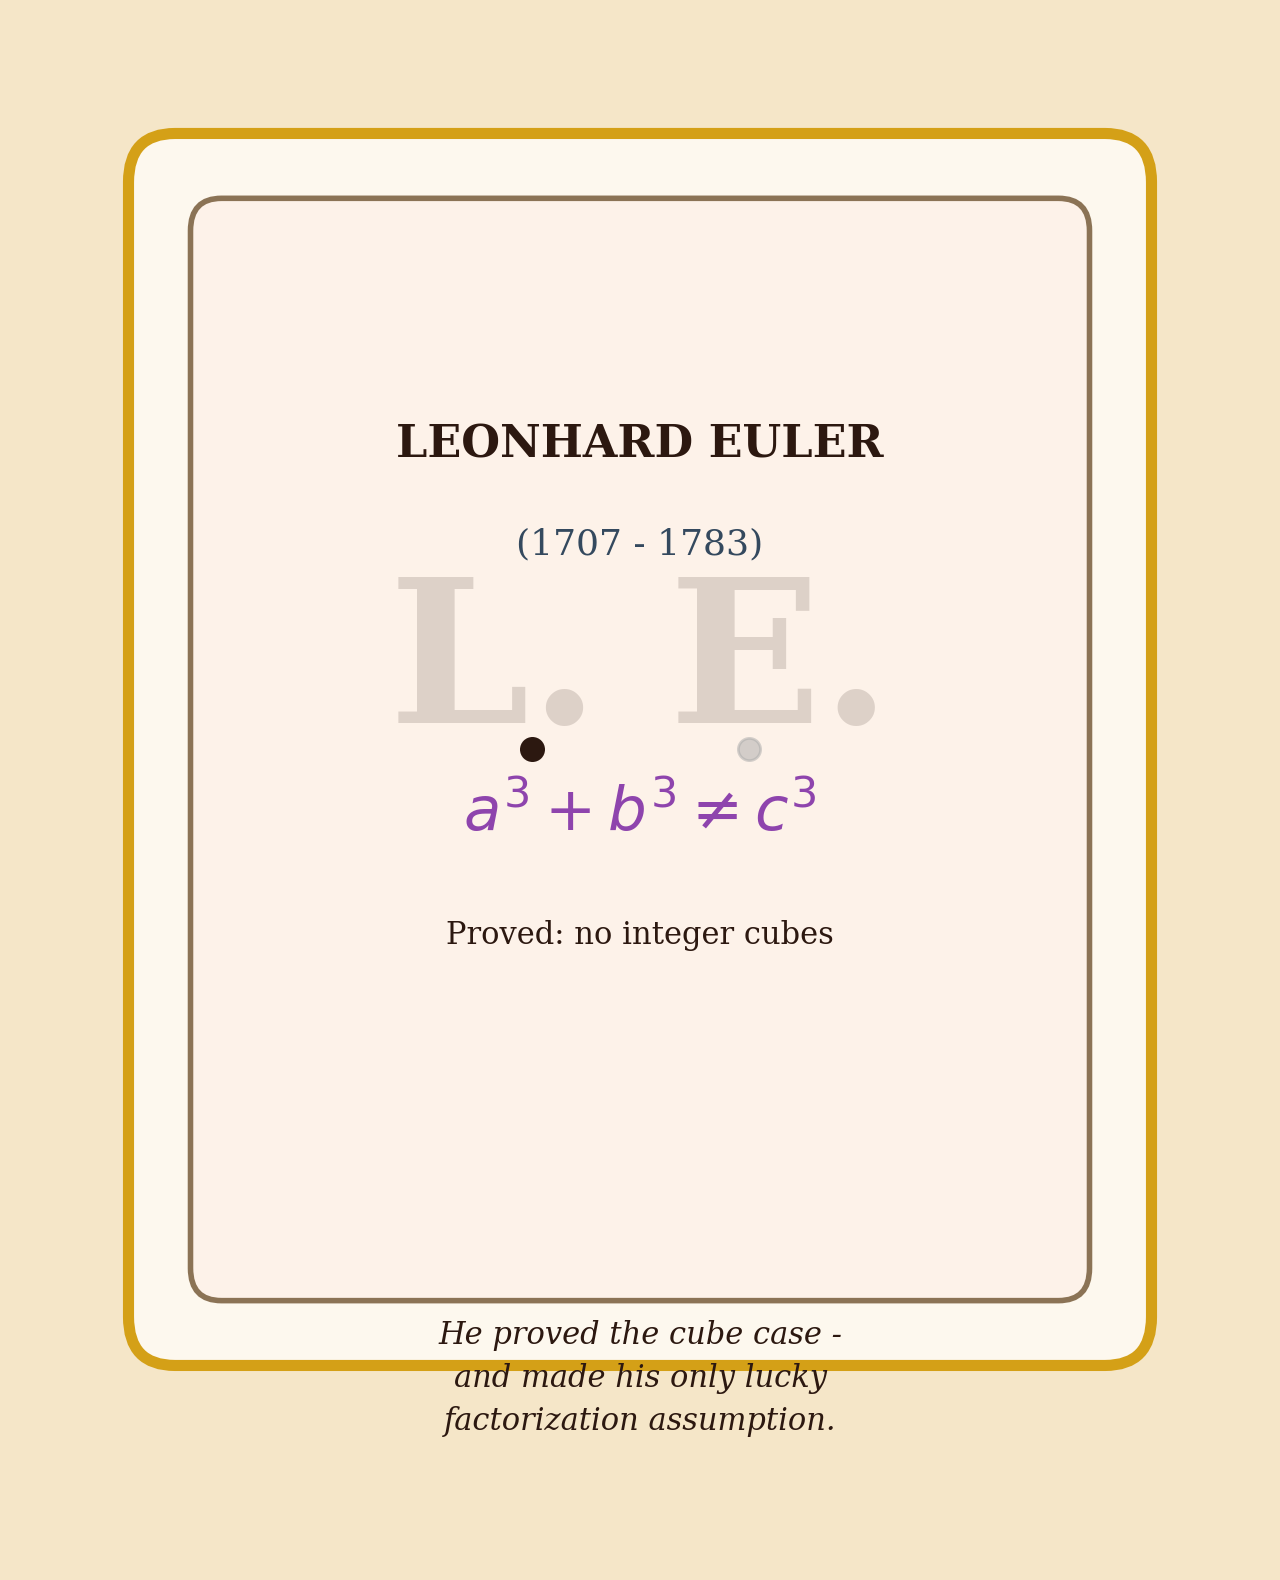
\includegraphics[width=0.85\textwidth]{Chapter10/images/fig08_euler_portrait.png}
\caption{}
\end{figure}
A portrait sketch of Leonhard Euler in three-quarter profile, rendered in a warm, slightly idealized pencil style. He wears a cap and a fur-trimmed coat. His right eye is clear and sharp; his left is clouded (Euler was blind in one eye for much of his career, and fully blind at the end). Below the portrait: ``Leonhard Euler (1707--1783). He proved the cube case --- and made his only lucky factorization assumption.''{]}

The norm function \(N(\alpha) = |a + b\omega|^2 = a^2 - ab + b^2\) plays the role of ``size'' in the Eisenstein integers: it is always a non-negative integer, it is multiplicative (\(N(\alpha\beta) = N(\alpha)N(\beta)\)), and it provides the staircase for the descent. Each step down shrinks the norm, and since the norm is a positive integer, the descent must terminate. The architecture of the proof mirrors Fermat's descent for \(n = 4\), but the arena has shifted from \(\mathbb{Z}\) to \(\mathbb{Z}[\omega]\) --- from a number line to a triangular lattice in the complex plane.

\bigskip\noindent\rule{\linewidth}{0.4pt}\bigskip

\section{The Unique Factorization Trap --- Why Fermat Was (Almost Certainly) Wrong}
Let us pause for a puzzle in an unfamiliar number system. Consider the integers of the form \(a + b\sqrt{-5}\), where \(a\) and \(b\) are ordinary integers. Call this ring \(\mathbb{Z}[\sqrt{-5}]\). Multiplication works as you would expect:

\[(1 + \sqrt{-5})(1 - \sqrt{-5}) = 1 - (-5) = 6,\]

and also \(6 = 2 \times 3\). So we have two genuinely different factorizations of \(6\):

\[6 = 2 \times 3 = (1 + \sqrt{-5})(1 - \sqrt{-5}).\]

None of these four factors --- \(2\), \(3\), \(1 + \sqrt{-5}\), \(1 - \sqrt{-5}\) --- can be broken down further in \(\mathbb{Z}[\sqrt{-5}]\). They are all ``irreducible.'' And yet they give \emph{different} factorizations of the same number. Unique factorization has failed.


\begin{figure}[htbp]
\centering
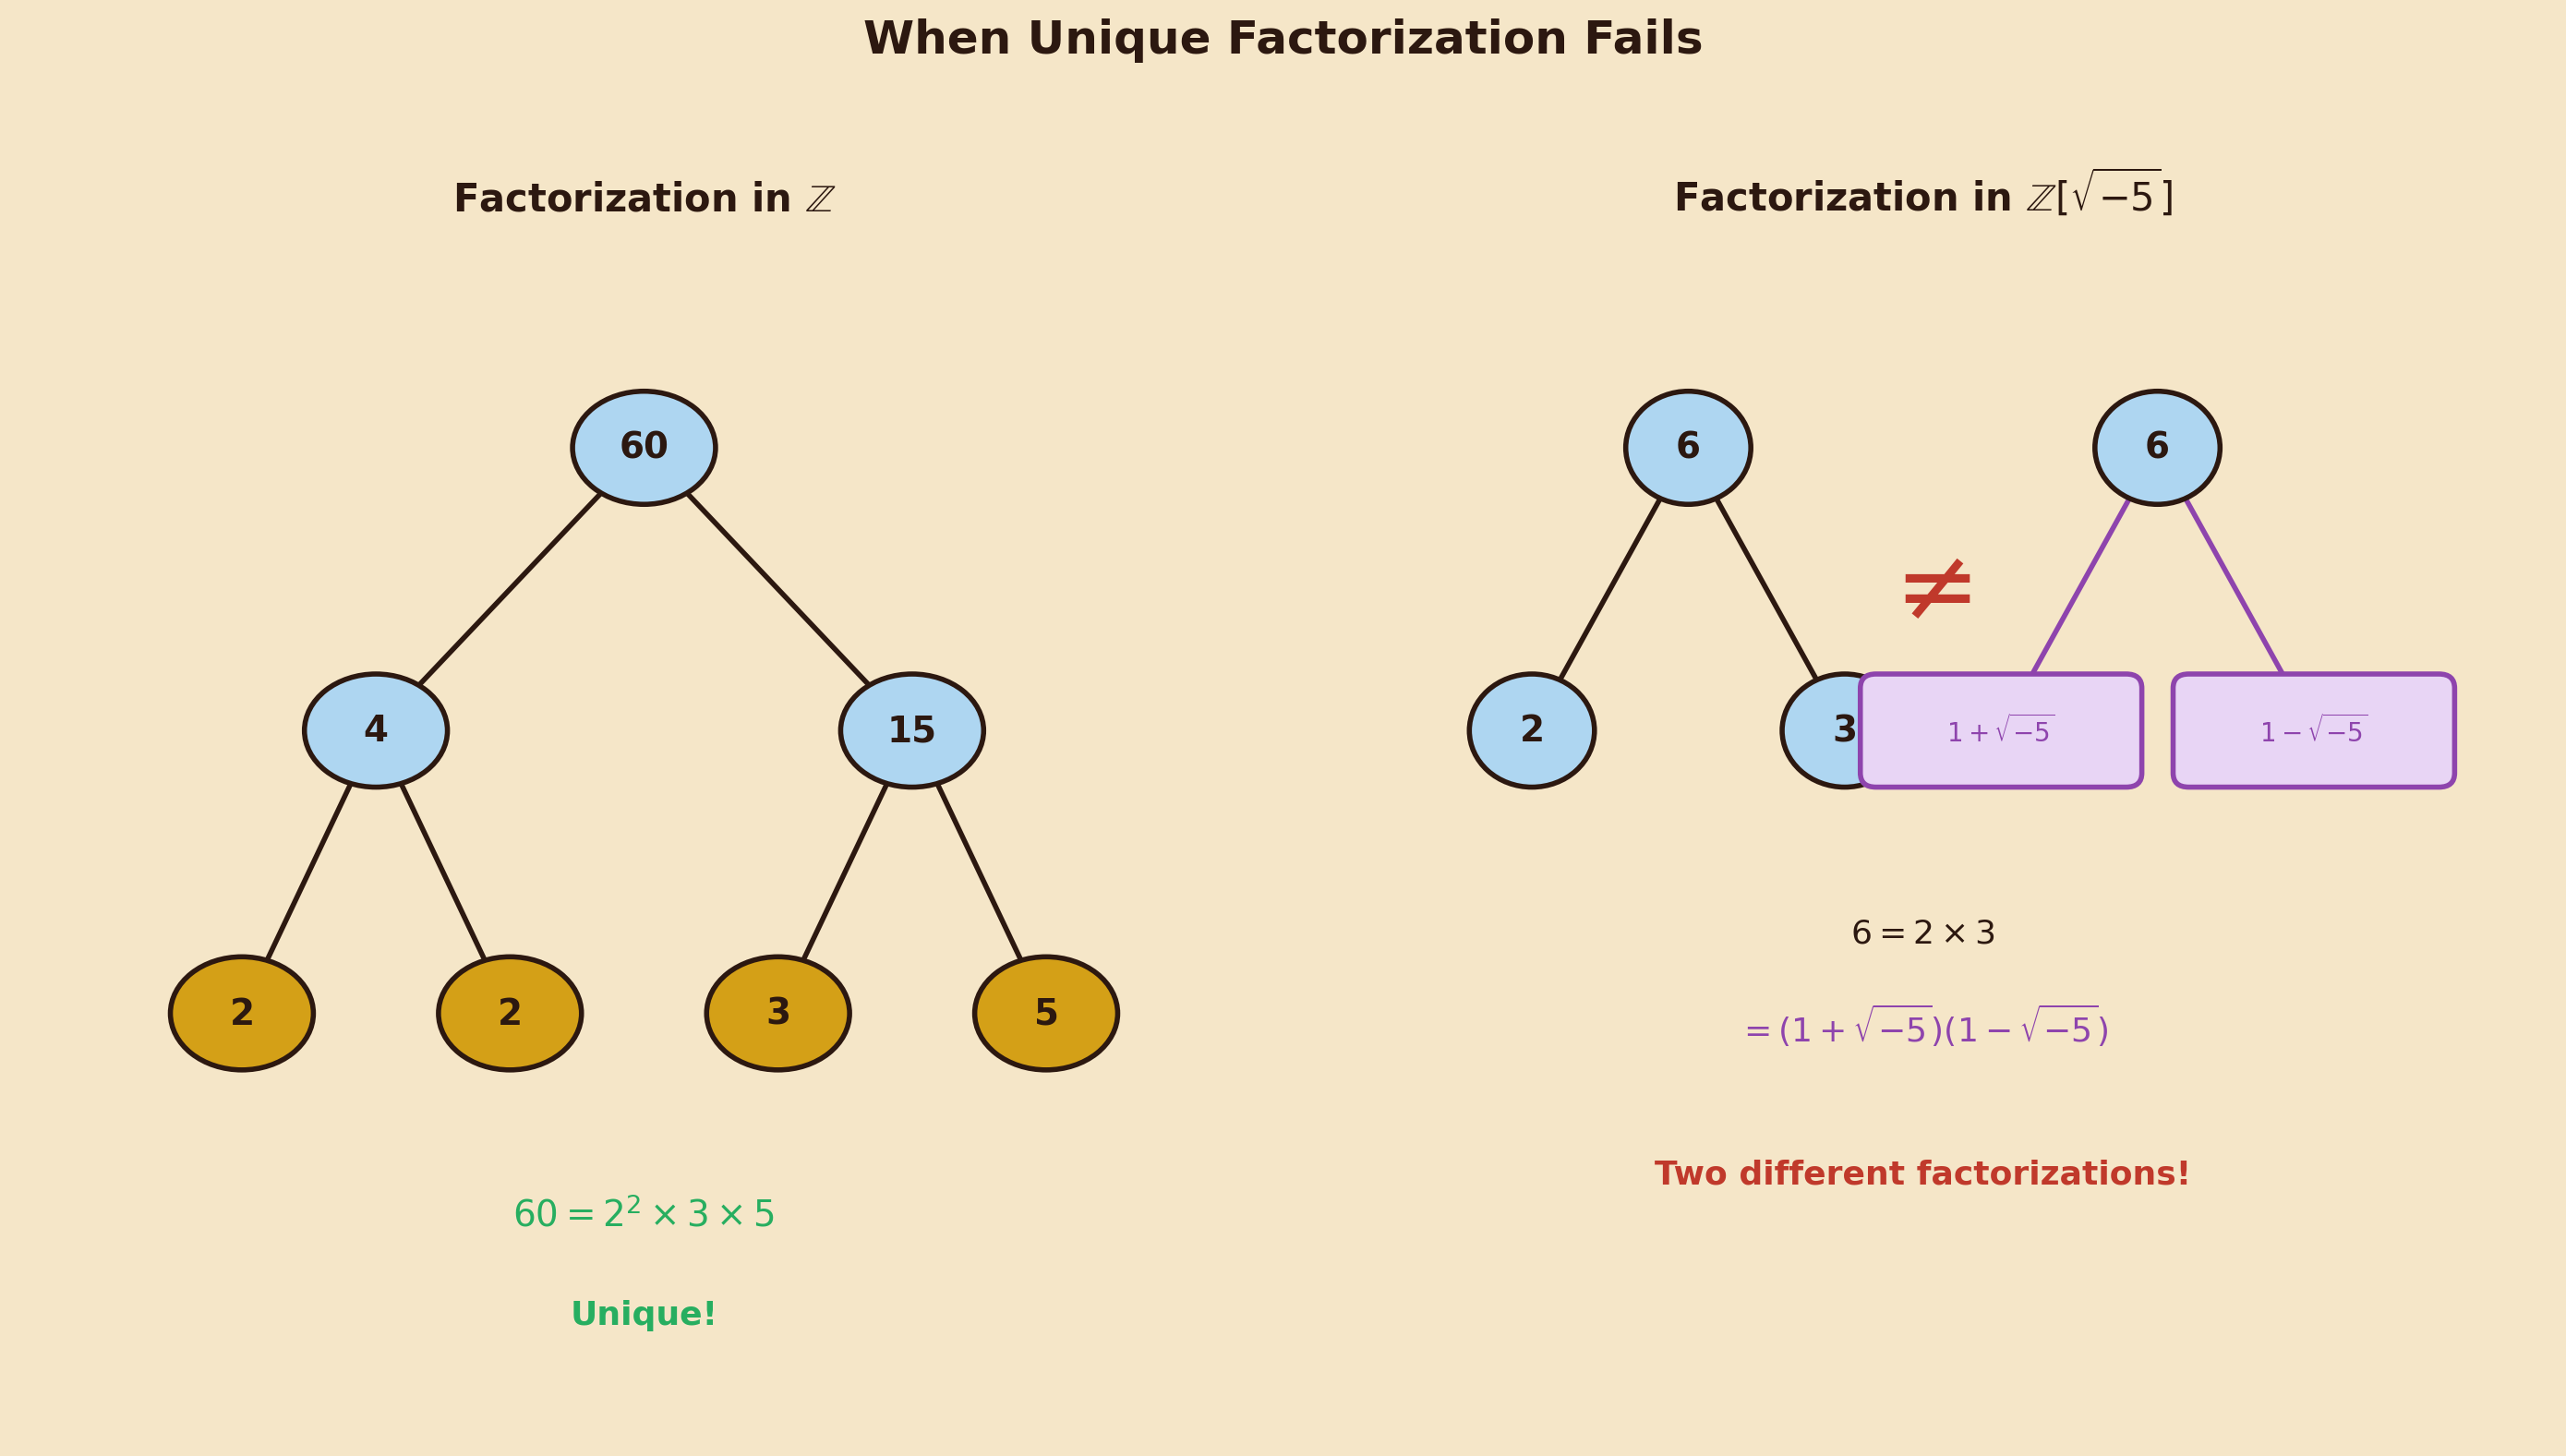
\includegraphics[width=0.85\textwidth]{Chapter10/images/fig09_factorization_comparison.png}
\caption{}
\end{figure}
A visual comparison of factorization in \(\mathbb{Z}\) versus \(\mathbb{Z}[\sqrt{-5}]\). On the left, a clean, unique factor tree for \(60 = 2^2 \times 3 \times 5\), with each branch terminating at a circled prime. On the right, two distinct factor trees for \(6\): one splitting into \(2 \times 3\), the other into \((1 + \sqrt{-5})(1 - \sqrt{-5})\). The two trees are drawn side by side with a large red ``\(\neq\)'' between them. The right-hand diagram is slightly tilted, as though the mathematical ground is unsteady.{]}

This is not an obscure pathology. It is a fundamental feature of algebraic number theory, and it is the reef on which the most natural approach to Fermat's Last Theorem founders.

Euler's proof for \(n = 3\) factored \(a^3 + b^3\) over \(\mathbb{Z}[\omega]\), where unique factorization happens to hold. But the same idea generalizes seductively. For any prime \(p\), let \(\zeta_p = e^{2\pi i/p}\) be a primitive \(p\)-th root of unity. Then the \textbf{cyclotomic integers} \(\mathbb{Z}[\zeta_p]\) are a natural number system in which \(a^p + b^p\) factors completely:

\[a^p + b^p = (a + b)(a + \zeta_p b)(a + \zeta_p^2 b) \cdots (a + \zeta_p^{p-1} b) = c^p.\]

If \(\mathbb{Z}[\zeta_p]\) has unique factorization, then each factor on the left must be a \(p\)-th power (up to units), and a descent argument finishes the job --- just as it did for \(p = 3\). This would prove FLT for all primes in one stroke.

There is only one problem: unique factorization fails in \(\mathbb{Z}[\zeta_p]\) for certain primes \(p\). The first failure occurs at \(p = 23\), as discovered by Ernst Kummer in 1847. The beautiful cyclotomic factorization, which works flawlessly for small primes, shatters against the rocks of arithmetic reality.

Kummer introduced the \textbf{class number} \(h(\mathbb{Q}(\zeta_p))\) as a measure of how badly unique factorization fails. When \(h = 1\), factorization is unique and the cyclotomic approach works perfectly. When \(h > 1\), there are distinct factorizations that cannot be reconciled, and the na"ive proof breaks down. He called a prime \(p\) \textbf{regular} if \(p\) does not divide the class number of \(\mathbb{Q}(\zeta_p)\), and proved FLT for all regular primes using a brilliant substitute for unique factorization: the theory of \textbf{ideal numbers}, the ancestor of the ideals that pervade modern algebra.

Here is a table of the first several primes and their regularity:

\begin{longtable}[]{@{}lll@{}}
\toprule\noalign{}
\(p\) & Regular? & Notes \\
\midrule\noalign{}
\endhead
\bottomrule\noalign{}
\endlastfoot
\(3\) & ✓ & Euler's proof works \\
\(5\) & ✓ & Dirichlet--Legendre \\
\(7\) & ✓ & Lamé \\
\(11\) & ✓ & \\
\(13\) & ✓ & \\
\(23\) & ✓ & First prime where \(h > 1\), but \(p \nmid h\) \\
\(37\) & ✗ & First irregular prime! \\
\(59\) & ✗ & \\
\(67\) & ✗ & \\
\end{longtable}

The irregular primes --- \(37, 59, 67, \ldots\) --- were the stubborn hold-outs that resisted Kummer's method. To handle them required entirely new mathematics, mathematics that would not be invented for another century and a half.


\begin{figure}[htbp]
\centering
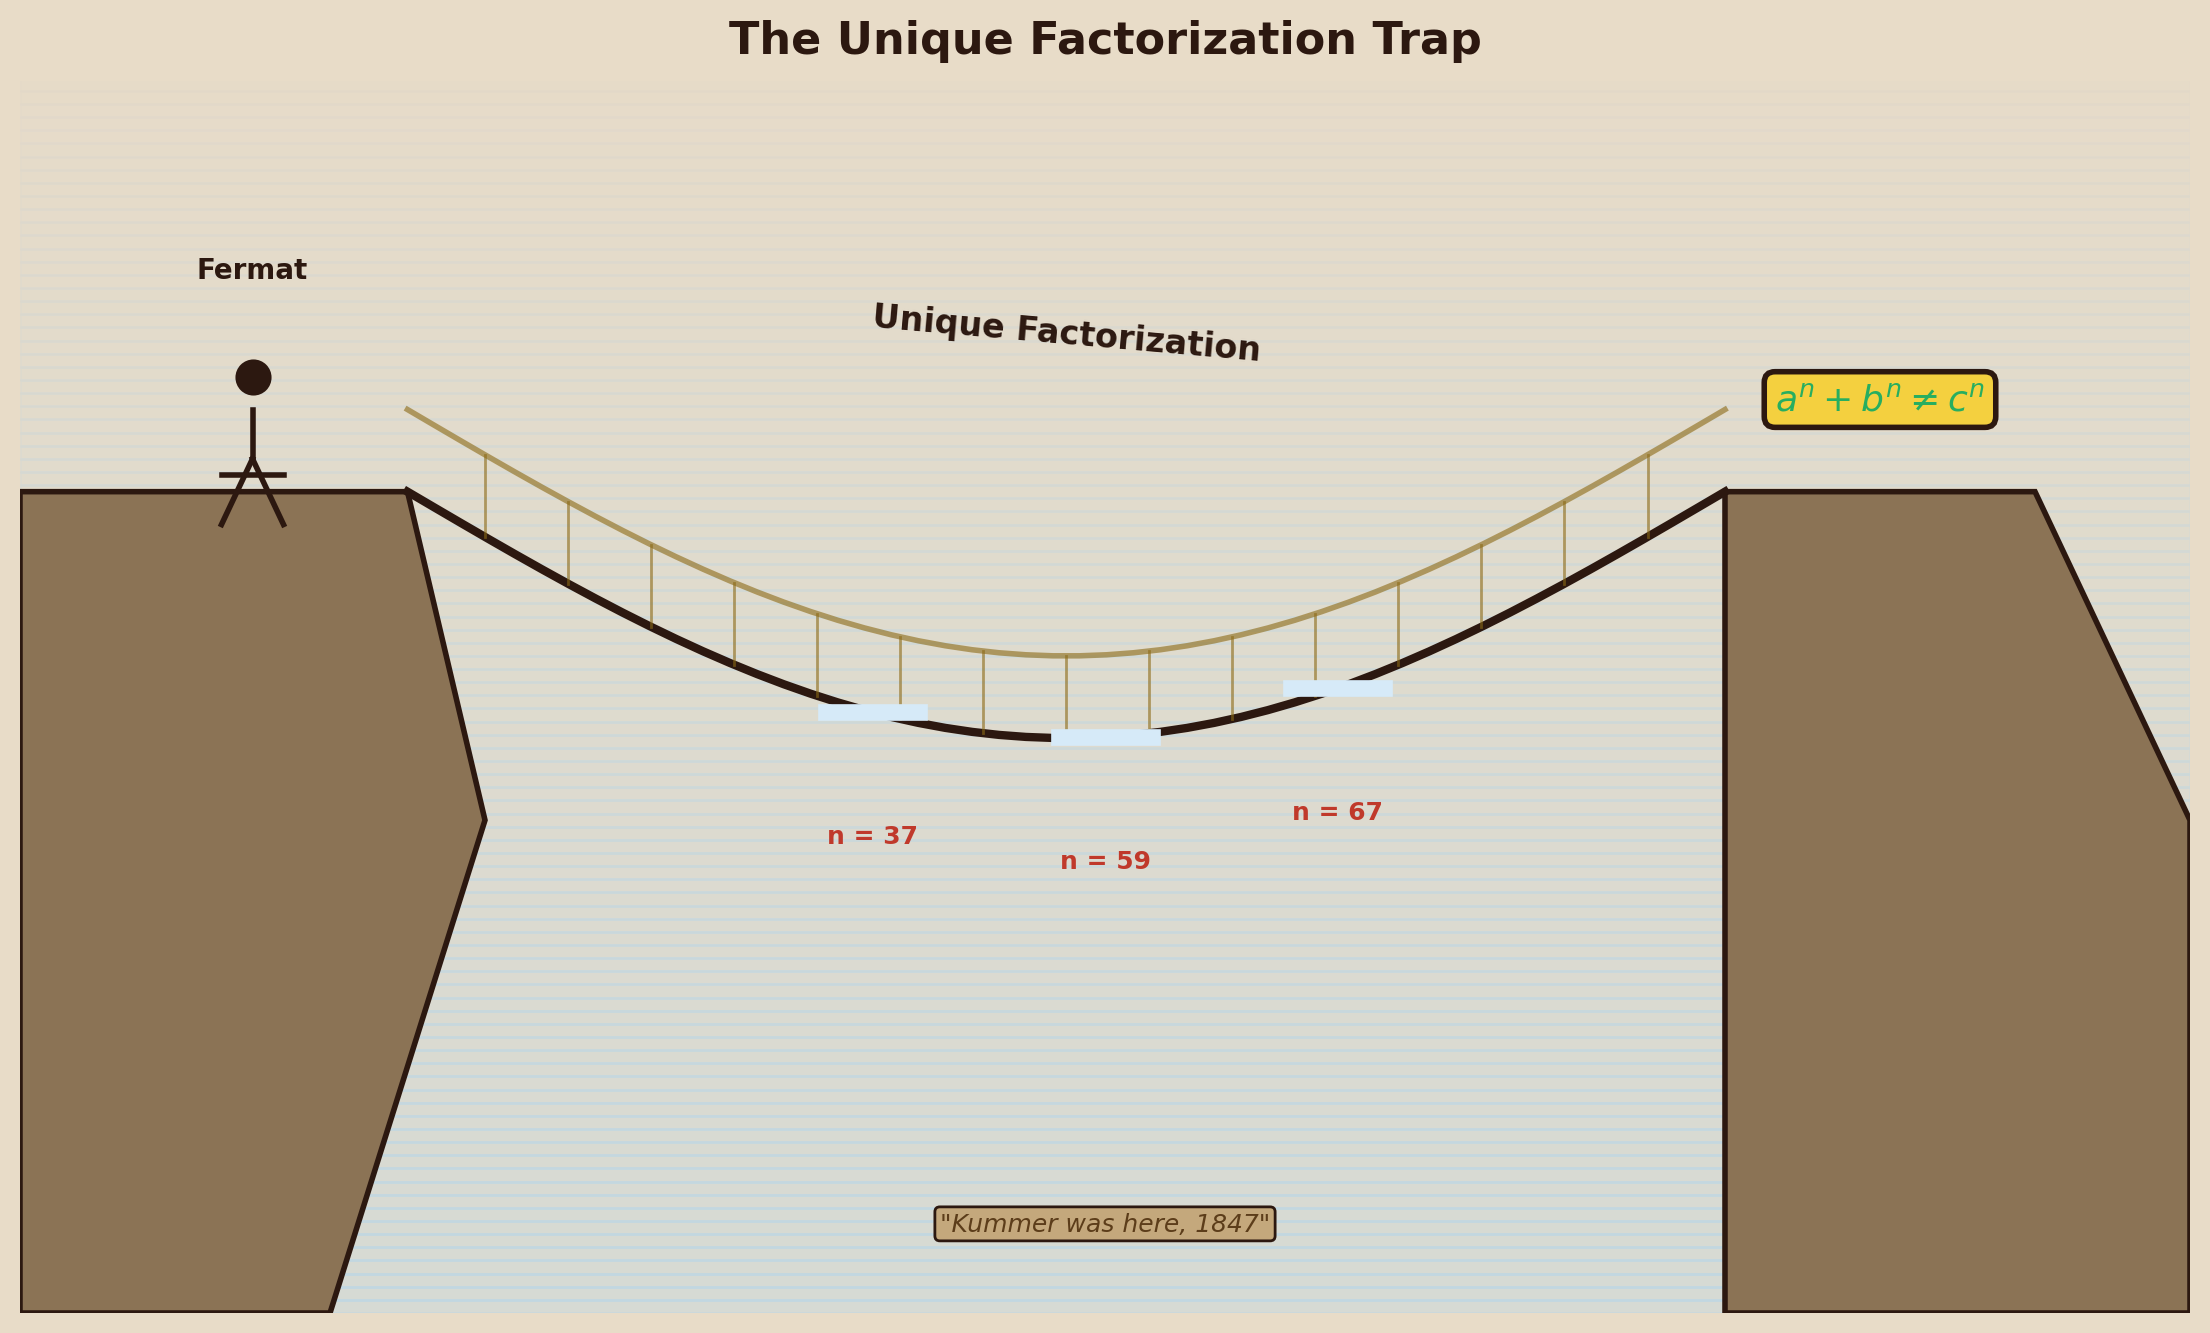
\includegraphics[width=0.85\textwidth]{Chapter10/images/fig10_uf_trap.png}
\caption{}
\end{figure}
A conceptual diagram of ``the unique factorization trap.'' A rope bridge labeled ``Unique Factorization'' spans a deep chasm between two cliffs. On the left cliff stands a figure resembling Fermat, confidently stepping onto the bridge with a rolled-up parchment under his arm. On the right cliff, across the bridge, glows the text ``\(a^n + b^n \neq c^n\) for all \(n\).'' But midway across the bridge, several planks are conspicuously missing, with the gaps labeled \(n = 37\), \(n = 59\), \(n = 67\). Far below in the chasm, a small wooden sign reads ``Kummer was here, 1847.'' The style is reminiscent of a Victorian adventure illustration.{]}

\textbf{What of Fermat himself?} Did he really have a proof? Almost certainly not --- or at least, not a correct one. The most plausible reconstruction is that Fermat had in mind a cyclotomic factorization argument, or something spiritually similar, that tacitly assumed unique factorization in the relevant number system. For small exponents (\(n = 3, 4, 5\)), this assumption happens to be true, and the proof goes through. But for \(n = 37\) --- or sooner, depending on the precise approach --- the assumption fails, and no amount of cleverness can patch it without Kummer's machinery, which would not exist for another two hundred years. Fermat claimed a proof; what he almost certainly had was a beautiful idea that works in special cases and breaks in general. The margin was not too small. The idea was too optimistic.

\bigskip\noindent\rule{\linewidth}{0.4pt}\bigskip

\section{What Would Fit in a Margin? --- An Inventory of Elementary Proofs}
If Fermat's proof of \(n = 4\) fits on a single page, how long would a complete elementary proof of FLT be? Let us take inventory.

\begin{longtable}[]{@{}llll@{}}
\toprule\noalign{}
Exponent \(n\) & Prover & Year & Approximate length \\
\midrule\noalign{}
\endhead
\bottomrule\noalign{}
\endlastfoot
\(4\) & Fermat & \$\sim\$1640 & \(\sim\) 1 page \\
\(3\) & Euler & 1770 & \(\sim\) 5 pages \\
\(5\) & Dirichlet \& Legendre & 1825 & \(\sim\) 15 pages \\
\(7\) & Lamé & 1839 & \(\sim\) 20 pages \\
\end{longtable}

Each new exponent required not just more pages, but genuinely new ideas. The proof for \(n = 5\) introduced quadratic reciprocity and careful analysis of units. The proof for \(n = 7\) pushed the algebraic machinery to its breaking point. There was no assembly line; each case was a custom-built siege engine aimed at a particular wall.


\begin{figure}[htbp]
\centering
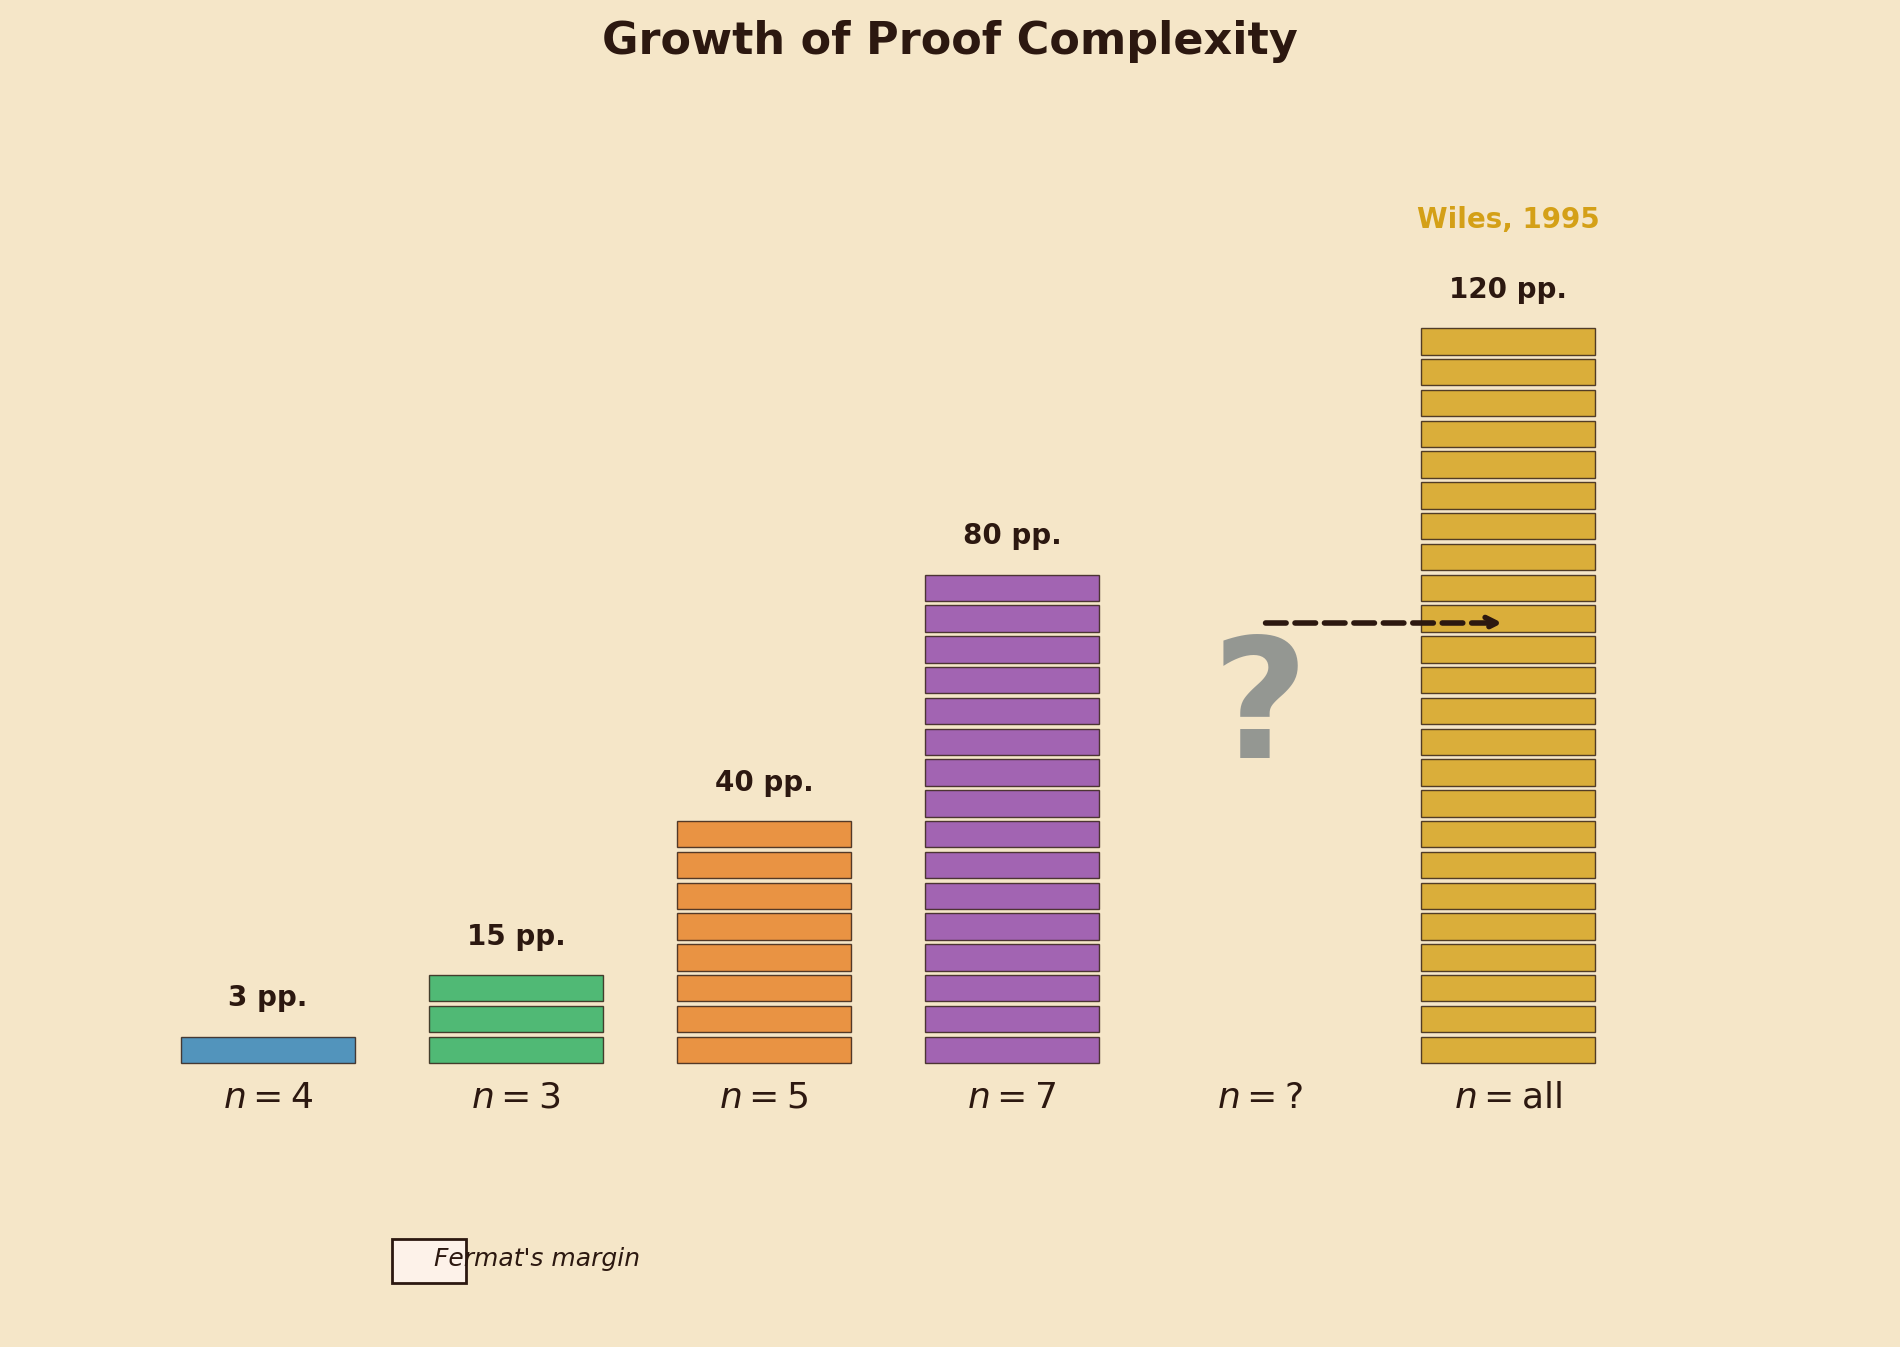
\includegraphics[width=0.85\textwidth]{Chapter10/images/fig11_proof_lengths.png}
\caption{}
\end{figure}
A bar chart showing the growth in proof length for FLT at exponents \(n = 4, 3, 5, 7\). The bars are drawn as stacks of manuscript pages, growing taller and more precarious with each exponent. After \(n = 7\), the bars are replaced by a towering question mark that extends off the top of the page, rendered in a comically tall, wobbly font. A dotted line from the question mark projects to a final bar labeled ``\(n = \text{all}\): \$\textgreater\$100 pages (Wiles, 1995).'' At the bottom, a tiny margin-sized rectangle is shown for comparison, labeled ``Fermat's margin.''{]}

A remarkable advance came from \textbf{Sophie Germain}, one of the most formidable mathematicians of the early nineteenth century, who had to submit her early work to Gauss under the male pseudonym ``Monsieur LeBlanc'' because the \textquotesingle Ecole Polytechnique did not admit women. Germain proved FLT for a wide swath of exponents under an auxiliary condition: if \(p\) is a prime such that \(2p + 1\) is \emph{also} prime (a condition now satisfied by the ``Germain primes'' \(2, 3, 5, 11, 23, 29, 41, \ldots\)), then the ``first case'' of FLT --- the case where none of \(a\), \(b\), \(c\) is divisible by \(p\) --- holds for exponent \(p\). Her criterion:

\[\text{If } p \text{ and } 2p+1 \text{ are both prime, and } x^p + y^p + z^p \equiv 0 \pmod{2p+1} \implies (2p+1) \mid xyz,\]

\[\text{then the first case of FLT holds for } p.\]


\begin{figure}[htbp]
\centering
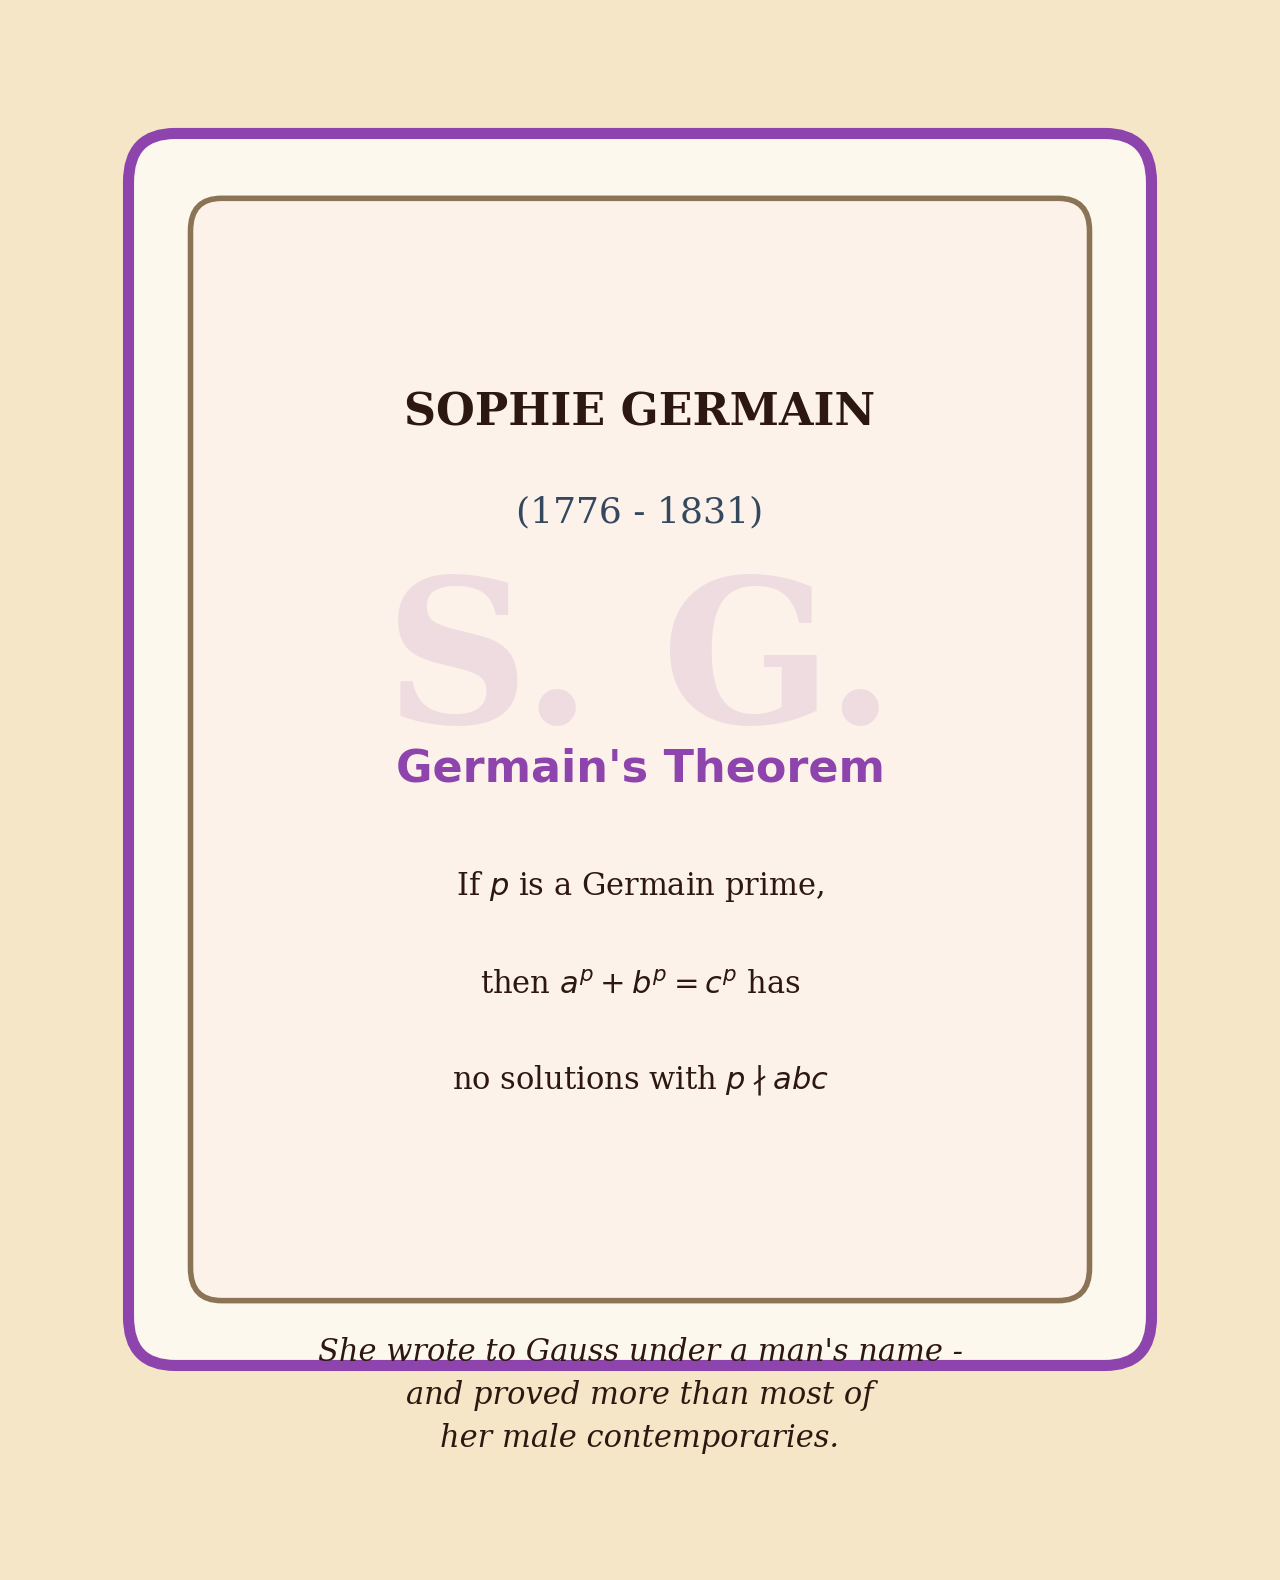
\includegraphics[width=0.85\textwidth]{Chapter10/images/fig12_germain_portrait.png}
\caption{}
\end{figure}
A portrait sketch of Sophie Germain, rendered in a soft pencil style. She is depicted in early 19th-century dress, with an intelligent, determined expression. Below the portrait: ``Sophie Germain (1776--1831). She wrote to Gauss under a man's name --- and proved more than most of her male contemporaries.''{]}

By the mid-twentieth century, computers had verified FLT for all exponents \(n < 4{,}000{,}000\). This was impressive engineering but unsatisfying mathematics. No matter how many cases you check, infinity lies beyond. The problem demanded not a bigger computer but a conceptual revolution.

\bigskip\noindent\rule{\linewidth}{0.4pt}\bigskip

\section{The Bridge from Geometry to Arithmetic --- Elliptic Curves and Modularity}
Draw a curve. Not a circle, not a parabola, but a \emph{cubic} --- say, \(y^2 = x^3 - x\). Plot it in the \(xy\)-plane and you will see two graceful arcs: one a smooth oval in the second quadrant, the other an undulating curve stretching to infinity on the right. Now mark two points with rational coordinates --- say \(P = (0, 0)\) and \(Q = (1, 0)\) --- and draw the straight line through them. This line will hit the curve at a third point \(R\), which also has rational coordinates. Reflect \(R\) across the \(x\)-axis, and call the result \(P + Q\). You have just performed \emph{addition} on an elliptic curve.


\begin{figure}[htbp]
\centering
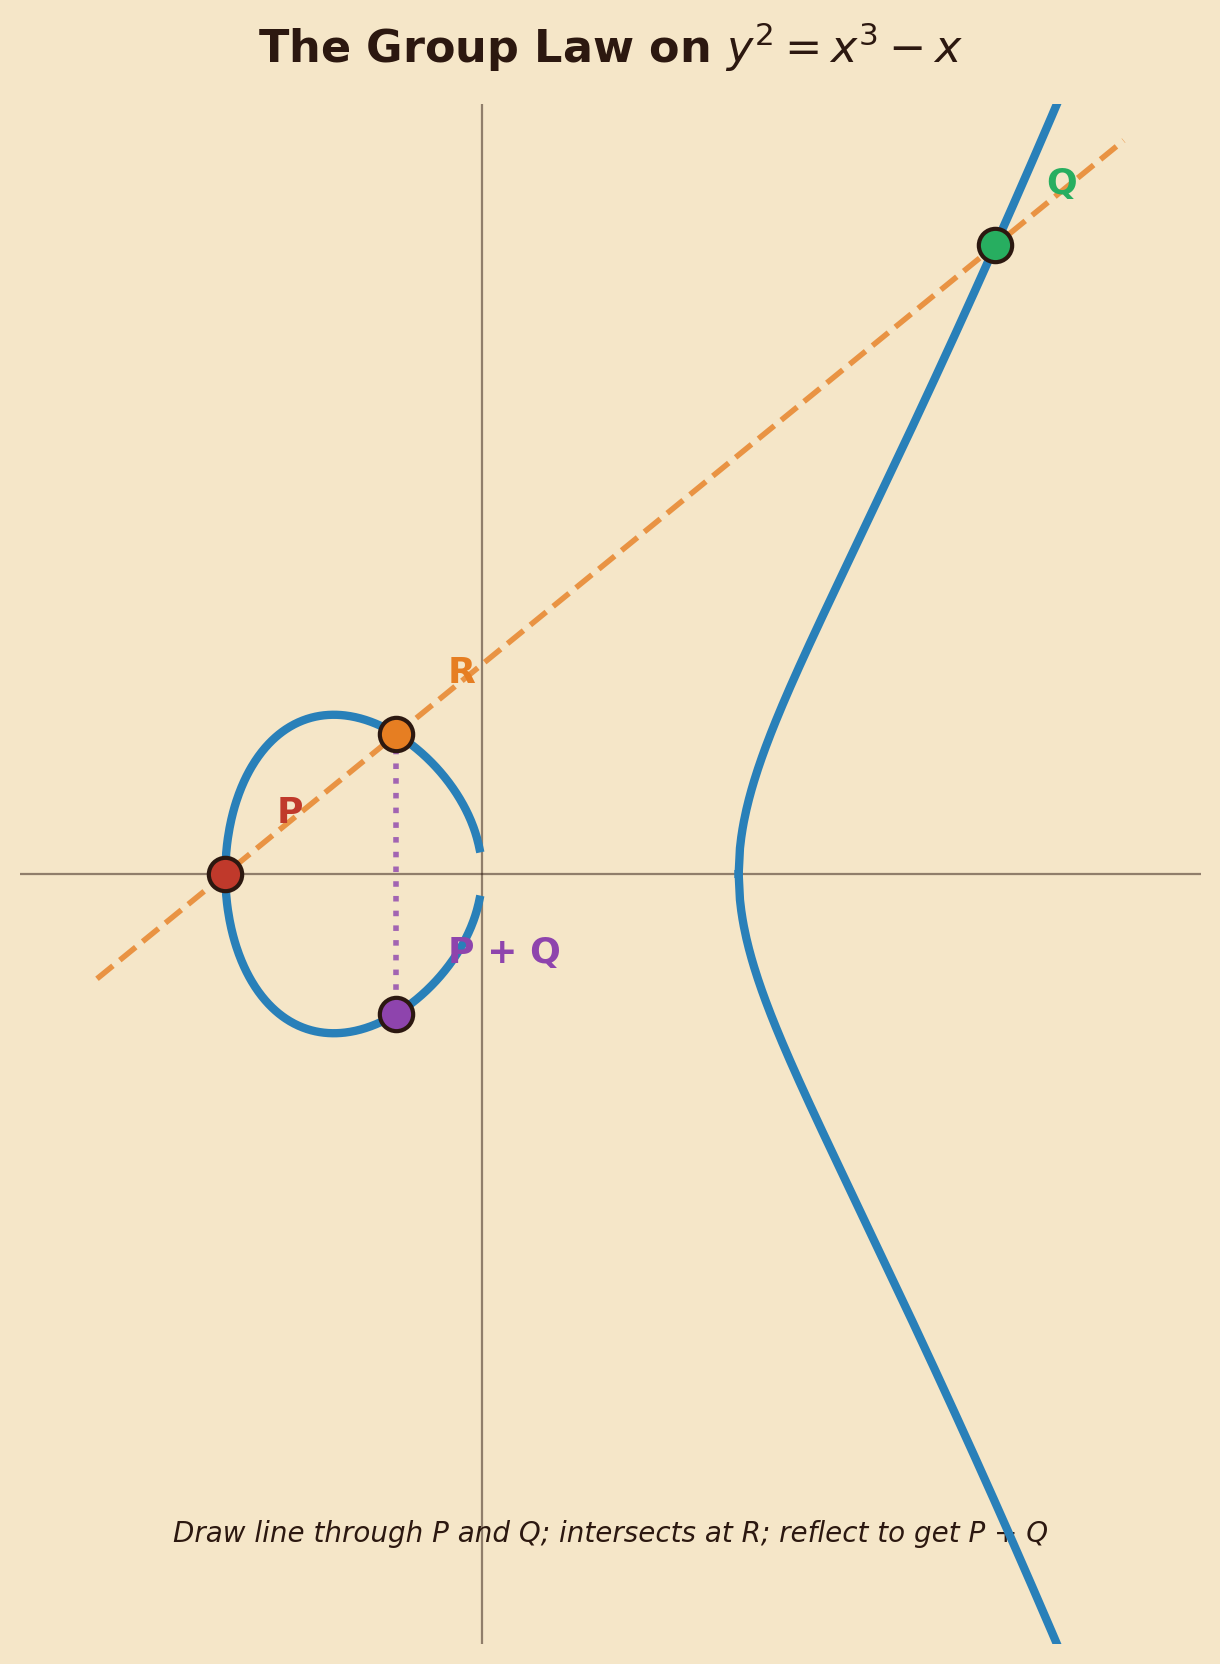
\includegraphics[width=0.85\textwidth]{Chapter10/images/fig13_elliptic_curve.png}
\caption{}
\end{figure}
A smooth cubic curve \(y^2 = x^3 - x\) plotted in the \(xy\)-plane, showing its two connected components. Two rational points \(P\) and \(Q\) are marked with dots. A straight line through \(P\) and \(Q\) intersects the curve at a third point \(R\). A vertical dashed line from \(R\) reflects it to the point \(P + Q\) on the other branch. Arrows and labels clearly show the geometric group operation. The axes are lightly drawn; the curve itself is bold and elegant.{]}

This geometric trick --- the chord-and-tangent law --- endows the rational points of an elliptic curve with the structure of an abelian group. You can add points, subtract them, double them, and so on, all by drawing lines. It is one of the most beautiful collisions of algebra and geometry in all of mathematics. But what on earth does the geometry of cubic curves have to do with Fermat's equation?

The answer arrived in 1985, from an unexpected direction. The German mathematician Gerhard Frey observed that if \((a, b, c)\) were a solution to \(a^p + b^p = c^p\) for some odd prime \(p\), then one could attach to this solution a specific elliptic curve --- now called the \textbf{Frey curve}:

\[E_{a,b,c} : \quad y^2 = x(x - a^p)(x + b^p).\]

This is a perfectly legal cubic equation. Its discriminant --- a measure of how ``singular'' the curve is --- works out to

\[\Delta = (abc)^{2p} / 2^8,\]

a quantity of such extreme arithmetic structure (a perfect \(2p\)-th power, divided by a power of \(2\)) that the resulting curve would be a monster among elliptic curves, a creature of bizarre and impossible properties.

At this point, a grand conjecture enters the story. In 1955, the Japanese mathematicians Yutaka Taniyama and Goro Shimura, later joined by Andr\textquotesingle e Weil, put forth the \textbf{modularity conjecture}: every elliptic curve over \(\mathbb{Q}\) is \emph{modular}, meaning that its arithmetic data --- the sequence of numbers \(a_n\) counting solutions modulo each prime --- matches the Fourier coefficients of a \emph{modular form}, a function of extraordinary symmetry defined on the upper half of the complex plane. The conjecture proposed that the world of algebraic geometry (elliptic curves) and the world of complex analysis (modular forms) are secretly the same world:

\[\sum_{n=1}^{\infty} a_n q^n \quad \text{is a weight-2 eigenform for } \Gamma_0(N).\]

In 1986, Kenneth Ribet proved the decisive link: \emph{the Frey curve, if it existed, could not be modular.} Its conductor --- a measure of where the curve has bad behavior --- would have a form incompatible with the known structure of modular forms. Ribet's theorem said: no modular form can match the Frey curve's arithmetic.

The chain of reasoning is now breathtaking in its clarity:

\begin{enumerate}
\def\labelenumi{\arabic{enumi}.}
\tightlist
\item
  Suppose \(a^p + b^p = c^p\) has a solution.
\item
  Form the Frey curve \(E_{a,b,c}\).
\item
  By Ribet's theorem, \(E_{a,b,c}\) is \emph{not} modular.
\item
  But by the Taniyama--Shimura conjecture, \emph{every} elliptic curve is modular.
\item
  Contradiction. No solution exists.
\end{enumerate}


\begin{figure}[htbp]
\centering
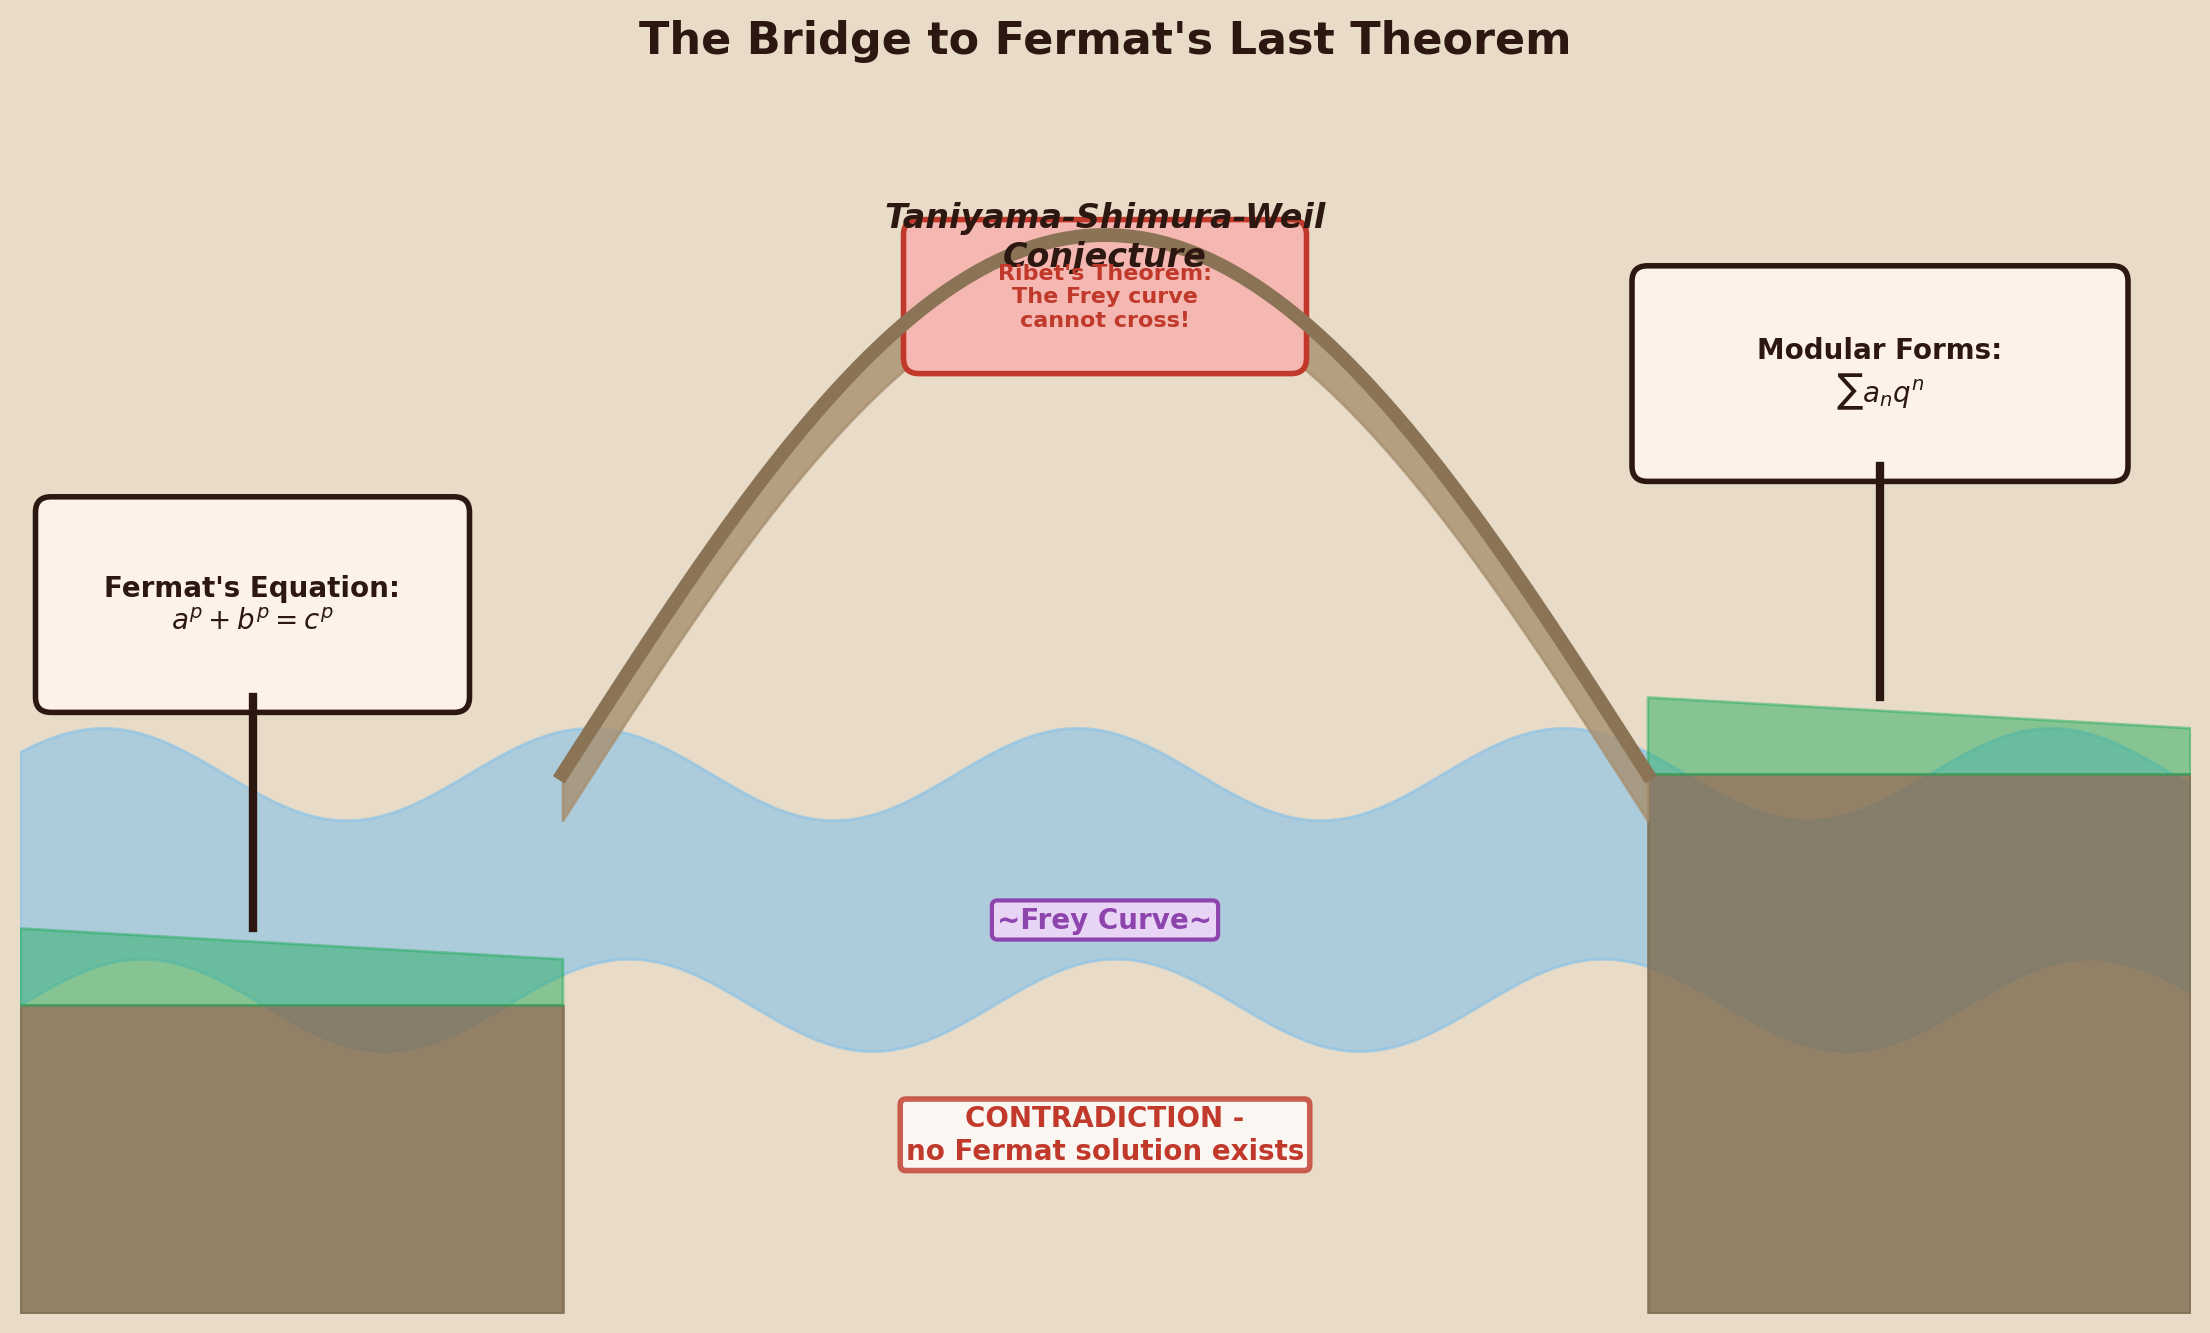
\includegraphics[width=0.85\textwidth]{Chapter10/images/fig14_bridge_diagram.png}
\caption{}
\end{figure}
A conceptual ``bridge'' diagram spanning a river. On the left bank stands a signpost reading ``Fermat's Equation: \(a^p + b^p = c^p\).'' In the river, perched on a rock, is the ``Frey Curve,'' depicted as a strange, twisted cubic curve with wild self-intersections. On the right bank stands a signpost reading ``Modular Forms: \(\sum a_n q^n\).'' A grand stone bridge arches over the river, inscribed with ``Taniyama--Shimura--Weil Conjecture.'' Halfway across the bridge, a wooden barricade with a sign: ``Ribet's Theorem: The Frey curve cannot cross.'' Below, in the churning water: ``CONTRADICTION --- no Fermat solution exists.''{]}

Fermat's Last Theorem had been reduced to a statement about the symmetries of complex functions. Prove the modularity conjecture --- or at least enough of it to cover the Frey curve --- and FLT follows as a corollary.

\bigskip\noindent\rule{\linewidth}{0.4pt}\bigskip

\section{Wiles's Proof --- The Margin That Took 358 Years to Fill}
In 1963, a ten-year-old boy named Andrew Wiles walked into the public library in Cambridge, England, and found a book about Fermat's Last Theorem. He was captivated. ``I knew from that moment,'' he later said, ``that I would never let it go.'' He carried the problem with him through school, through university, through his early career --- always in the back of his mind, always waiting.

In 1986, when Ribet's theorem completed the bridge between FLT and the modularity conjecture, Wiles saw his chance. He retreated into secrecy. For seven years, he told almost no one what he was working on --- not his colleagues, not his students, not even his wife, until the final stages. He worked alone in an attic study, emerging only to teach his classes and maintain the appearance of a normal academic life.

On June 23, 1993, at a conference at the Isaac Newton Institute in Cambridge --- the same Cambridge where, thirty years earlier, a boy had found a book in a library --- Wiles delivered a series of three lectures. The title was deliberately vague: ``Modular Forms, Elliptic Curves, and Galois Representations.'' But the audience, filled with the world's leading number theorists, knew something extraordinary was coming. By the end of the third lecture, Wiles had outlined a proof of the modularity conjecture for \emph{semistable elliptic curves} --- the class that includes the Frey curve. He wrote the last line on the blackboard, set down his chalk, and said, quietly: ``I think I'll stop here.''

The room erupted. Newspapers around the world ran the headline: \textbf{FERMAT'S LAST THEOREM PROVED.}

And then --- disaster. During the refereeing process, a subtle gap was found in a crucial step of the argument. The edifice that had taken seven years to build was cracked. Wiles spent a year in anguish, trying and failing to repair the gap. He was on the verge of giving up when, in September 1994, working with his former student Richard Taylor, he found a completely different approach to the problematic step --- an approach that was, in its own way, even more elegant than the original. The proof was published in 1995, filling over 100 pages of the \emph{Annals of Mathematics}.

What did Wiles actually prove? At its heart, the proof establishes an isomorphism between two mathematical objects:

\[R \xrightarrow{\;\sim\;} \mathbf{T},\]

where \(R\) is a \textbf{universal deformation ring} --- a ring that parametrizes all the ways a certain Galois representation can be ``deformed'' --- and \(\mathbf{T}\) is a \textbf{Hecke algebra} --- an algebra that encodes the arithmetic of modular forms. This single isomorphism, known as the ``\(R = \mathbf{T}\)'' theorem, is the engine that drives the entire proof. It says that the algebraic deformations of a Galois representation are \emph{exactly} captured by the world of modular forms. Every deformation is modular; in particular, the one attached to any semistable elliptic curve is modular; in particular, the Frey curve (if it existed) would have to be modular; but Ribet proved it cannot be; so it does not exist; so Fermat's equation has no solutions.

The proof uses Galois representations, deformation rings, Hecke algebras, Selmer groups, the Taylor--Wiles patching method, and deep results from the arithmetic of modular forms. It is a tour de force of twentieth-century mathematics, drawing on almost every major development in number theory and algebraic geometry since Kummer.


\begin{figure}[htbp]
\centering
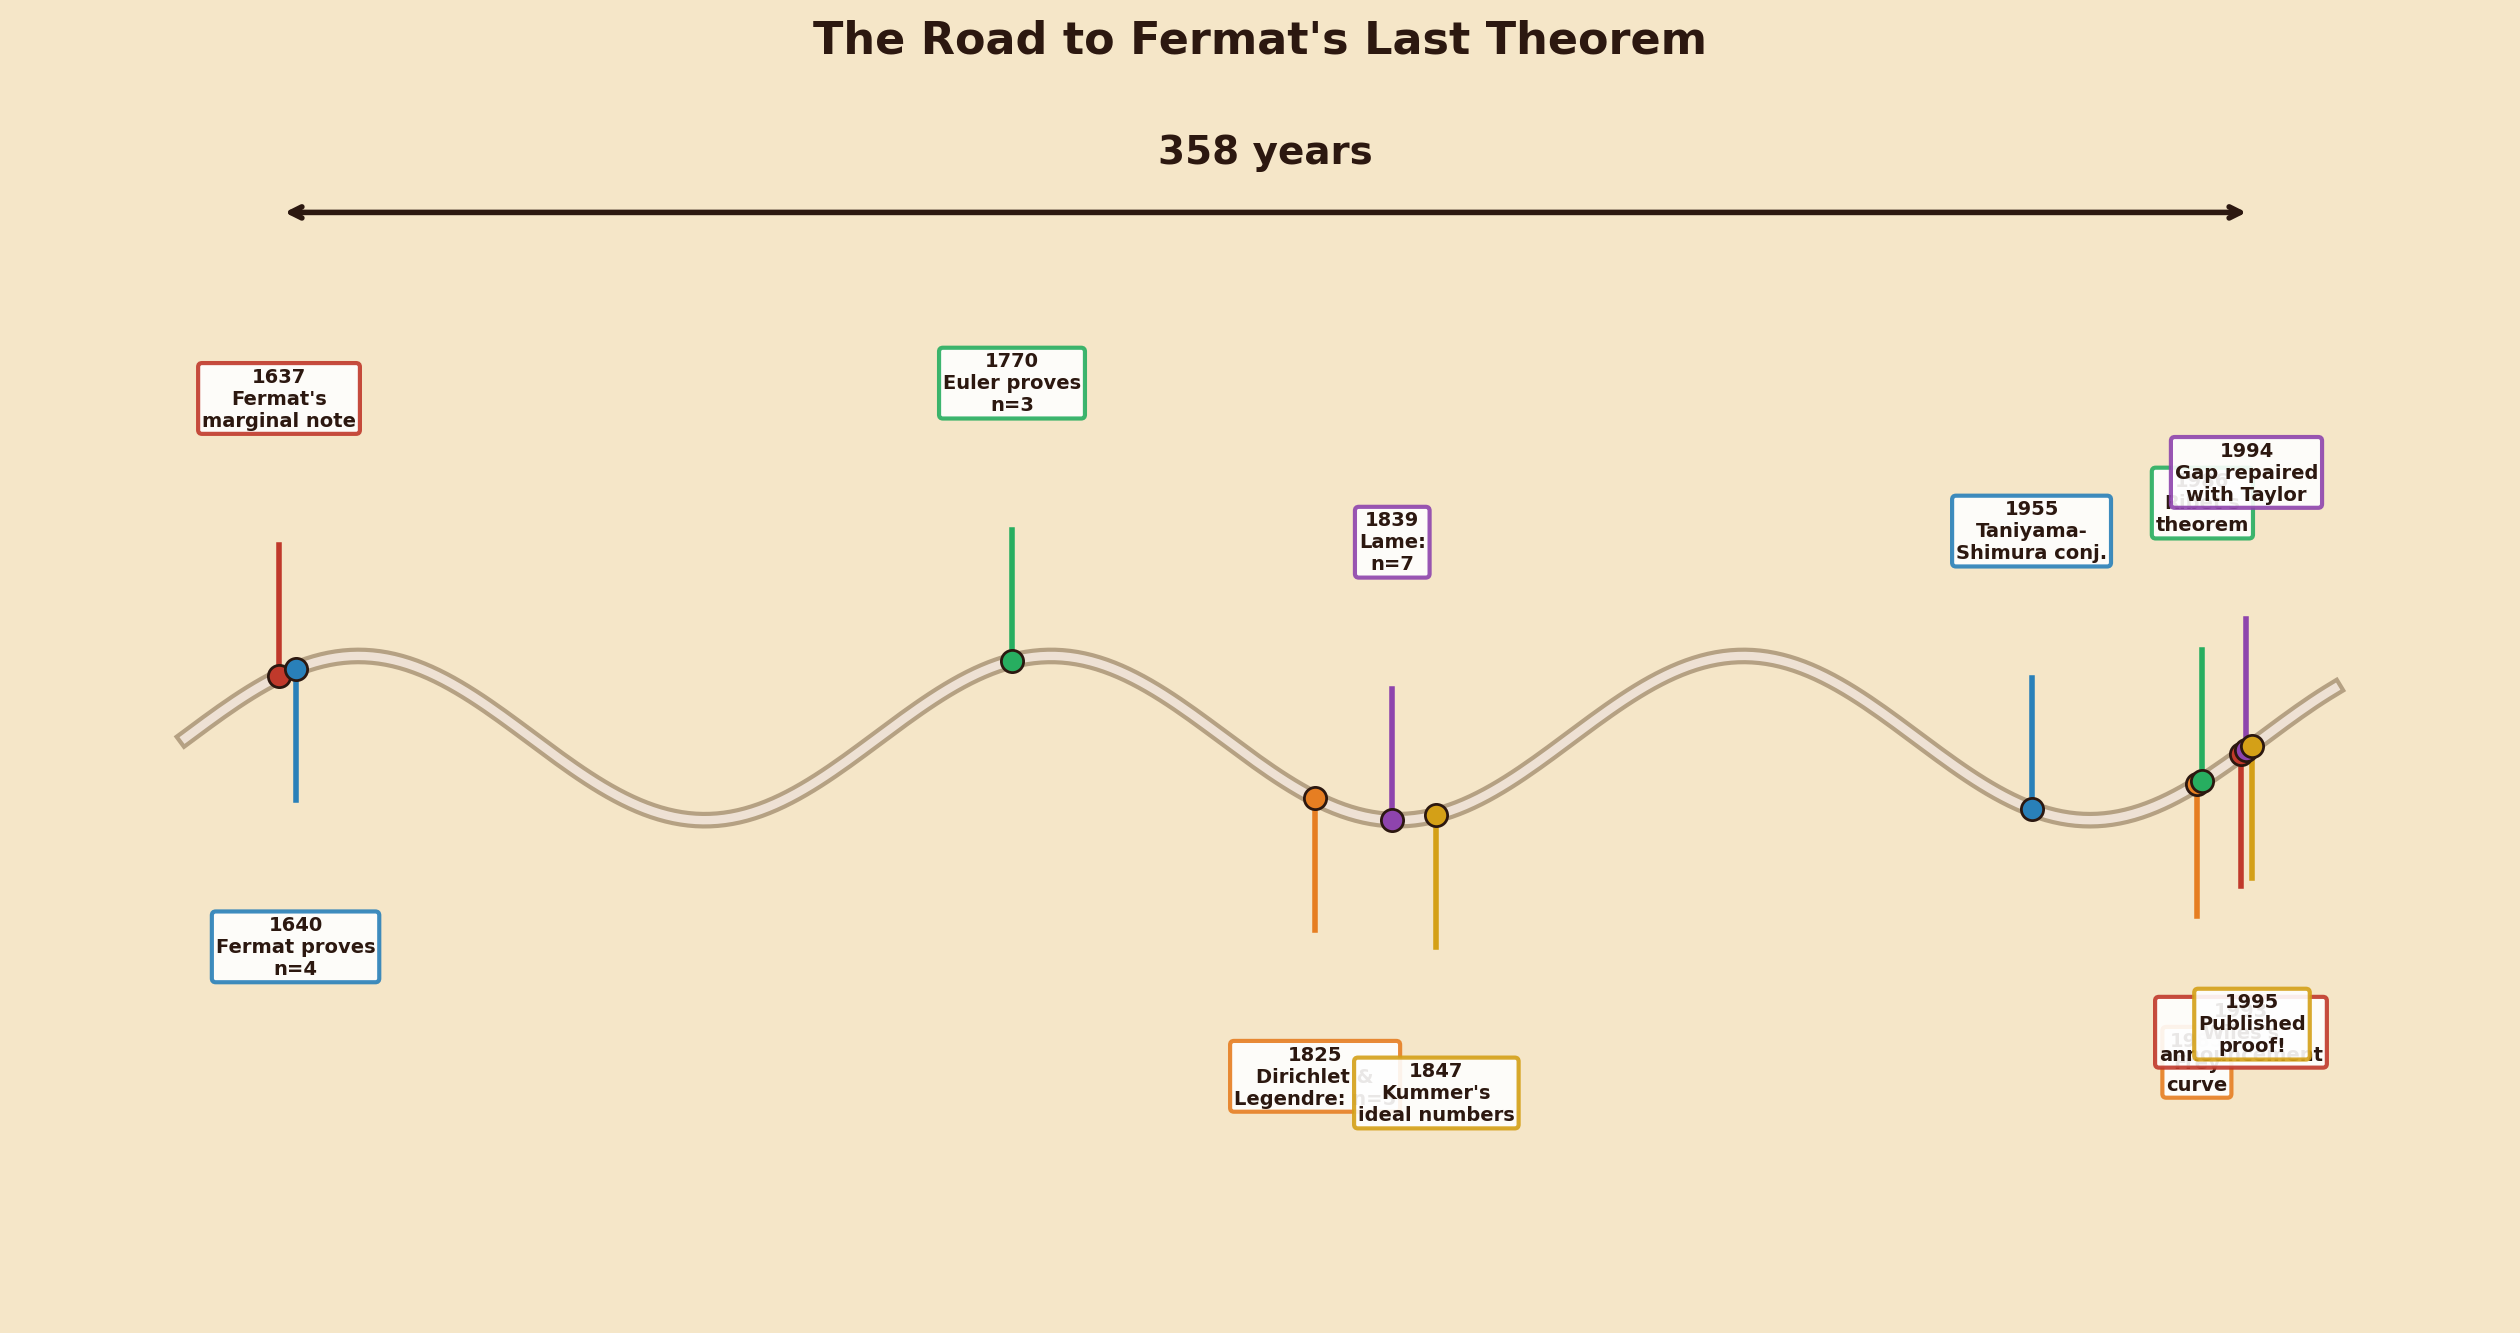
\includegraphics[width=0.85\textwidth]{Chapter10/images/fig15_timeline.png}
\caption{}
\end{figure}
A timeline stretching from 1637 to 1995, drawn as a winding road through a mountainous landscape. Key dates are marked with milestones: 1637 (Fermat's marginal note, depicted as a tiny book with a quill), \$\sim\$1640 (Fermat proves \(n = 4\), a small flag), 1770 (Euler proves \(n = 3\), a slightly larger flag), 1825 (\(n = 5\), Dirichlet \& Legendre), 1839 (\(n = 7\), Lamé), 1847 (Kummer's ideal numbers, a bridge over a gorge), 1955 (Taniyama--Shimura conjecture, a telescope pointed at a distant peak), 1985 (Frey curve, a strange rock formation), 1986 (Ribet's theorem, a signpost), 1993 (Wiles's announcement, a summit flag --- but with a crack in the ground), 1994 (gap repaired with Taylor, the crack sealed), 1995 (published proof, a golden summit marker). The 358-year span is emphasized by the road's immense length. The style evokes a hand-drawn explorer's map.{]}


\begin{figure}[htbp]
\centering
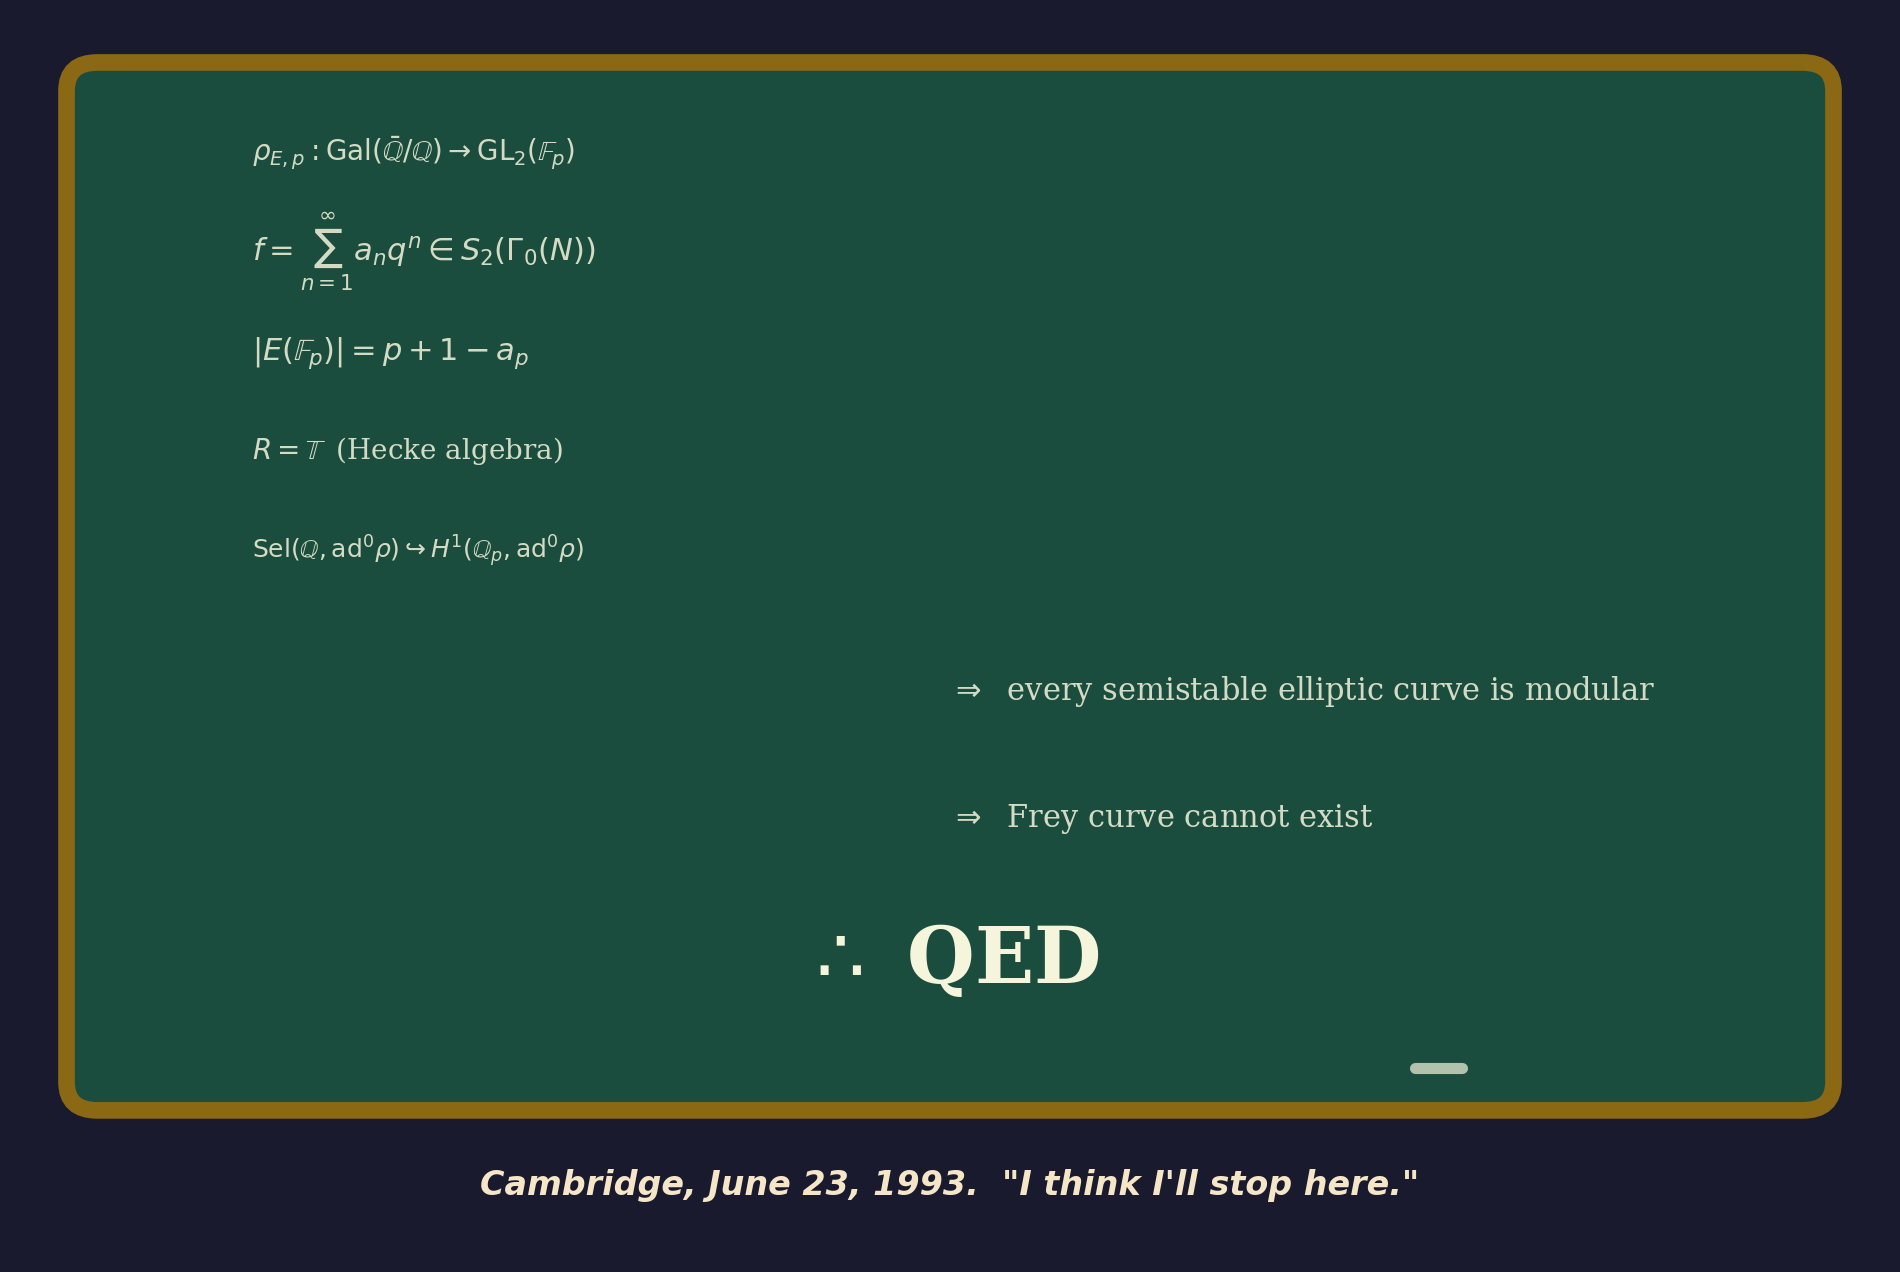
\includegraphics[width=0.85\textwidth]{Chapter10/images/fig16_blackboard.png}
\caption{}
\end{figure}
A photograph-style sketch of a blackboard covered in dense mathematical notation --- modular forms, Galois symbols, commutative diagrams --- with the final line reading ``\(\therefore\) QED'' in large chalk letters. A chalk-dusty hand is setting down a piece of chalk at the board's lower edge. The caption reads: ``Cambridge, June 23, 1993. `I think I'll stop here.'\,''{]}

Fermat claimed a proof that ``the margin was too narrow to contain.'' Wiles's proof fills over a hundred pages of dense mathematics, using theories and techniques invented two to three centuries after Fermat's death. The margin was not too small. The proof was too big --- because the mathematics it required had not yet been born.

\bigskip\noindent\rule{\linewidth}{0.4pt}\bigskip

\section{What Remains --- Open Frontiers and the Eternal Margin}
And now, one final puzzle. We know that \(a^n + b^n = c^n\) has no positive-integer solutions for \(n \ge 3\). End of story? Hardly. The landscape \emph{around} Fermat's Last Theorem is vast, wild, and largely uncharted. Let me offer you a few landmarks.

We know that two cubes cannot sum to a cube. But can two cubes sum to the \emph{same number} in two different ways? They certainly can:

\[1729 = 1^3 + 12^3 = 9^3 + 10^3.\]

This is the famous \textbf{taxicab number}, so named because of a story told by G. H. Hardy about visiting his brilliant collaborator Srinivasa Ramanujan in a London hospital. Hardy mentioned that his cab had borne the number 1729, which seemed to him rather dull. ``No, Hardy,'' Ramanujan replied instantly. ``It is a very interesting number. It is the smallest number expressible as the sum of two cubes in two different ways.'' The equation \(a^n + b^n = c^n + d^n\) is a close cousin of Fermat's equation, and its solutions are rich and mysterious.

What about \(a^4 + b^4 + c^4 = d^4\)? Euler conjectured that this was impossible --- a natural extension of FLT. The conjecture stood for over two centuries. Then, in 1988, Noam Elkies of Harvard shattered it with an explicit counterexample:

\[2{,}682{,}440^4 + 15{,}365{,}639^4 + 18{,}796{,}760^4 = 20{,}615{,}673^4.\]

So the prohibition against equal sums of powers is not as sweeping as one might hope. Fermat's equation is a special island of impossibility in a sea of subtle possibilities.

Several grand conjectures remain open. The \textbf{Beal Conjecture}, carrying a prize of one million dollars, asserts:

\[\text{If } a^x + b^y = c^z \text{ with } a, b, c, x, y, z \in \mathbb{Z}^+ \text{ and } x, y, z \ge 3, \text{ then } \gcd(a, b, c) > 1.\]

That is: if the exponents are all at least \(3\), then the bases must share a common factor. Fermat's Last Theorem is a special case (with \(x = y = z\) and the added requirement \(\gcd(a,b,c) = 1\), which is then impossible). The Beal Conjecture remains wide open.

Then there is the \textbf{\(abc\) conjecture}, formulated by Joseph Oesterl\textquotesingle e and David Masser in 1985. For a positive integer \(n\), define its \emph{radical} \(\mathrm{rad}(n) = \prod_{p \mid n} p\) --- the product of its distinct prime factors, each taken once. The conjecture states: for every \(\varepsilon > 0\), there are only finitely many coprime triples \((a, b, c)\) with \(a + b = c\) and

\[c > \mathrm{rad}(abc)^{1 + \varepsilon}.\]

This deceptively simple statement about the interplay between addition and multiplication has extraordinary consequences. It implies FLT for all sufficiently large \(n\) in essentially one line of argument. It implies the Beal Conjecture (with finitely many exceptions). It implies deep results about the distribution of primes. In 2012, Shinichi Mochizuki of Kyoto University posted a 500-page claimed proof; as of this writing, the mathematical community has not reached consensus on its correctness. The margin of understanding is, in this case, genuinely too narrow to contain the argument --- or perhaps the argument is too novel for the existing margins of the community's expertise.


\begin{figure}[htbp]
\centering
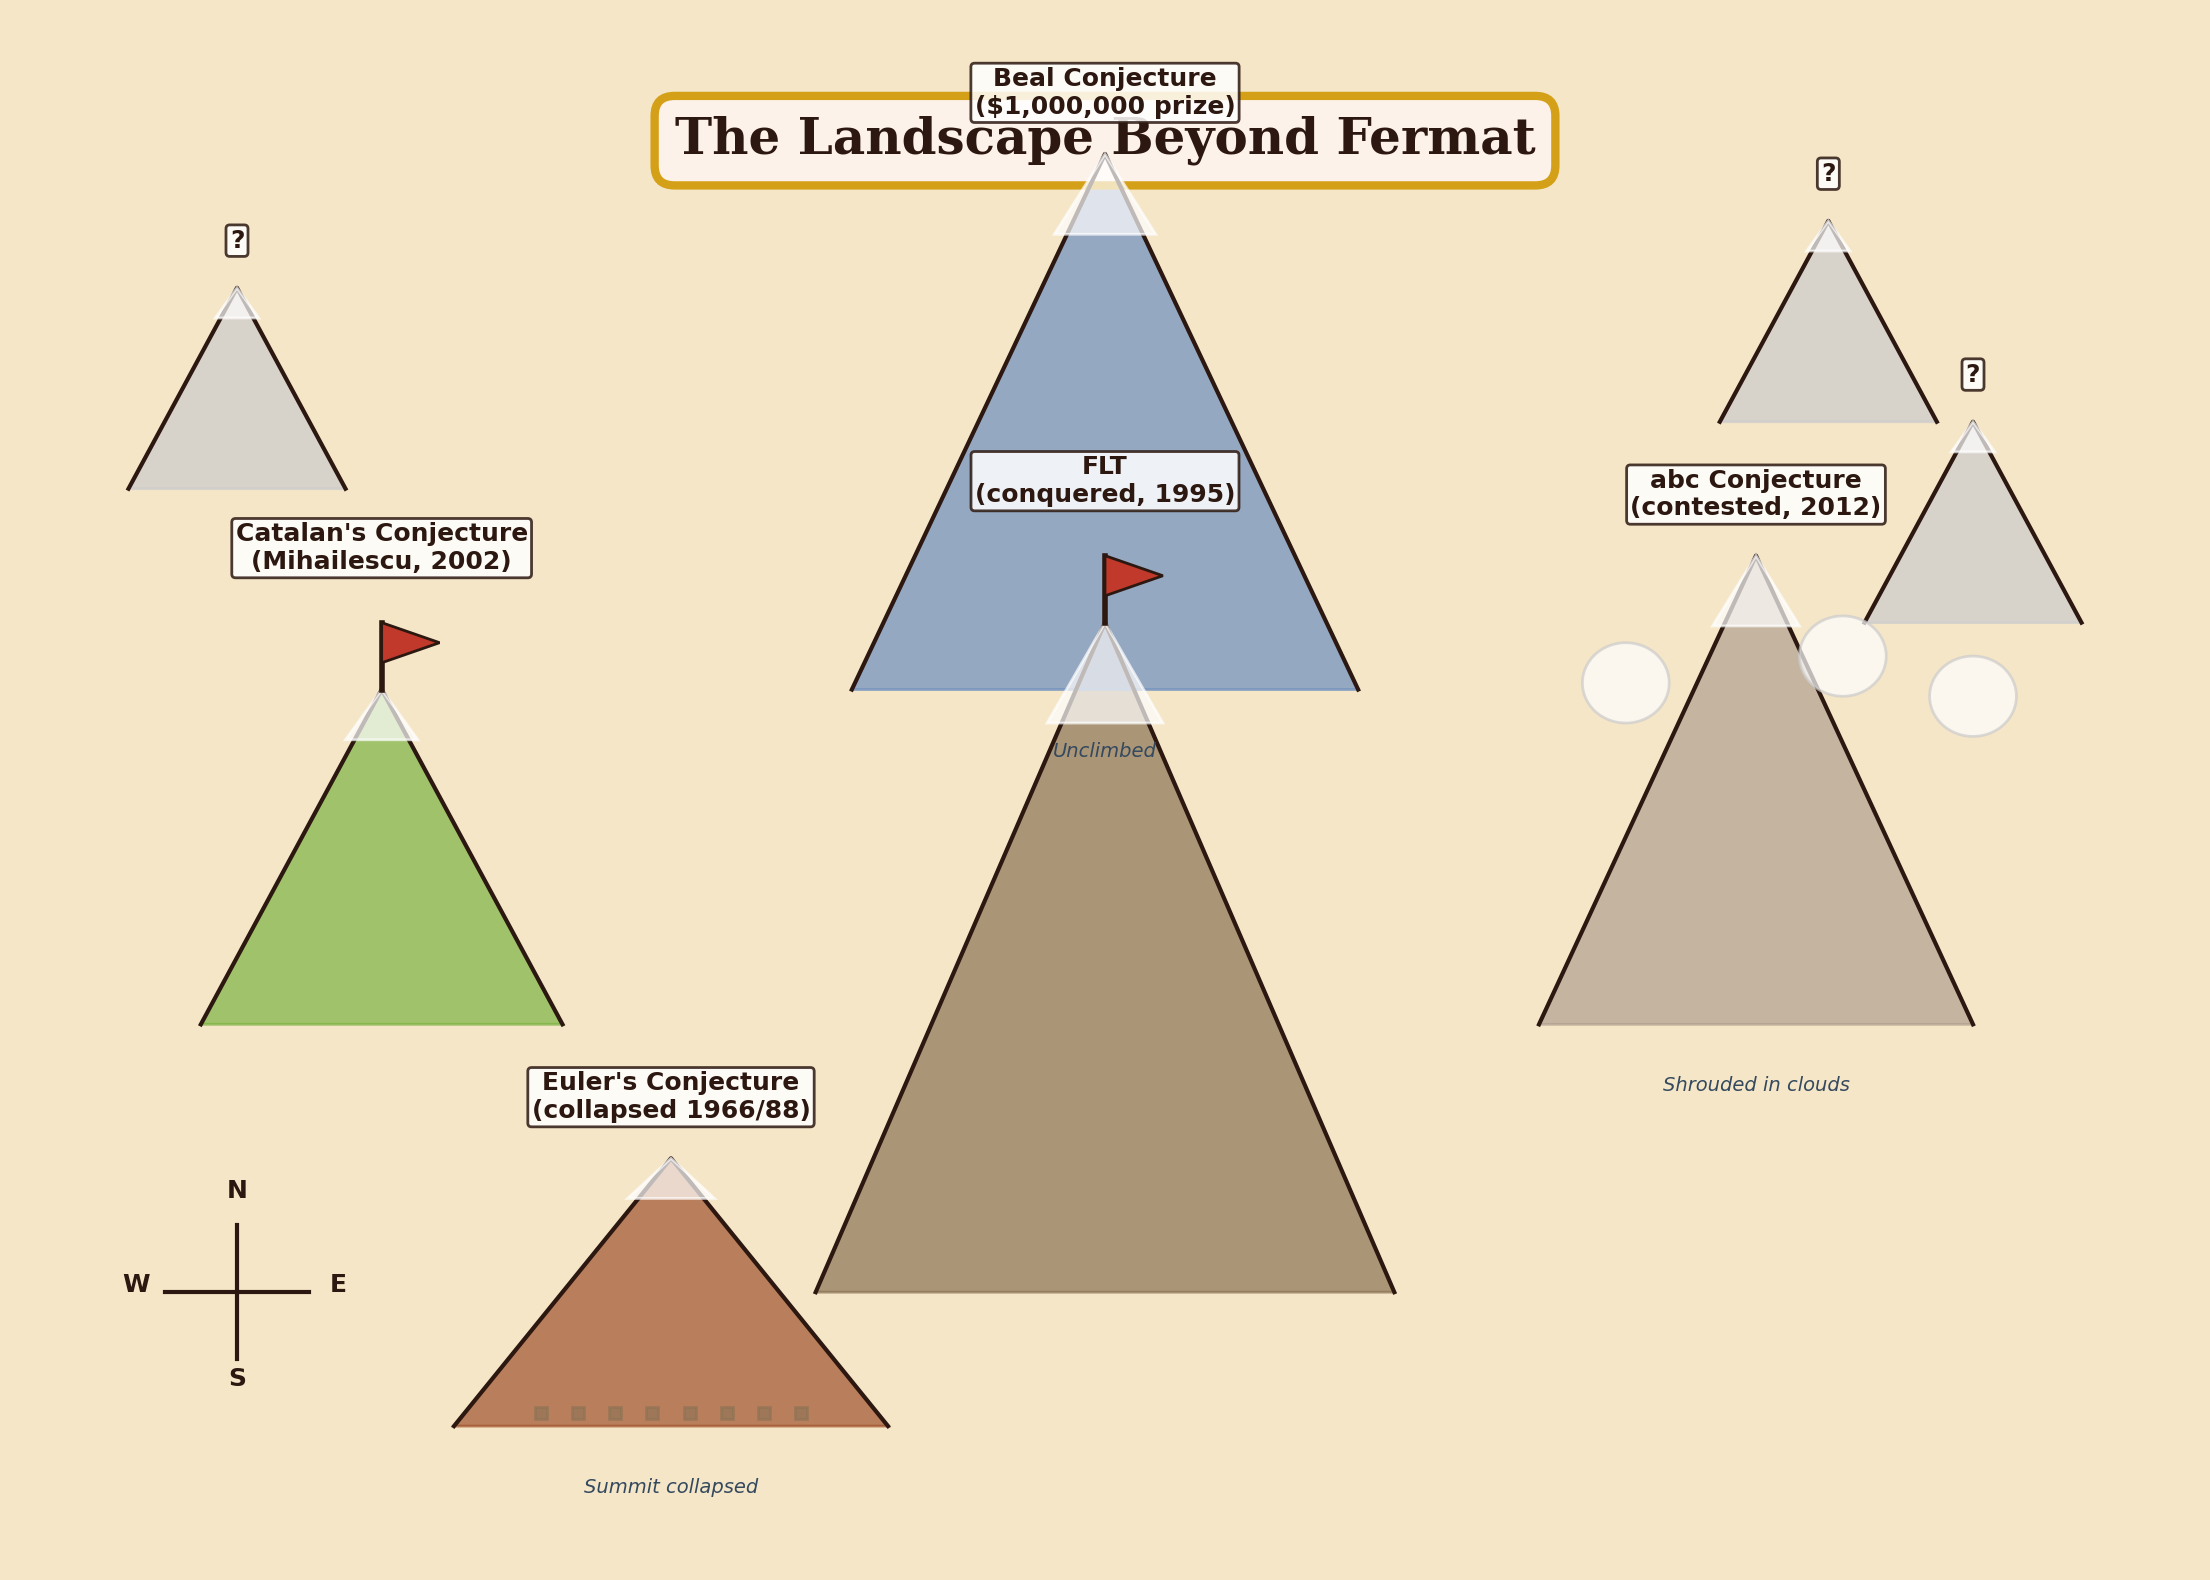
\includegraphics[width=0.85\textwidth]{Chapter10/images/fig17_landscape_beyond.png}
\caption{}
\end{figure}
A visual map labeled ``The Landscape Beyond Fermat.'' In the center, a tall mountain peak labeled ``FLT (conquered, 1995)'' flies a flag at its summit. Surrounding it in all directions: peaks of varying heights. To the north, a tall unclimbed peak labeled ``Beal Conjecture (\$1,000,000 prize).'' To the east, a peak shrouded in swirling clouds labeled ``\(abc\) Conjecture (contested route, 2012).'' To the south, a collapsed peak with rubble at its base labeled ``Euler's Conjecture (summit collapsed, 1966/1988).'' To the west, a smaller peak with a flag labeled ``Catalan's Conjecture (conquered by Mih\u{a}ilescu, 2002).'' Further peaks fade into mist, labeled with question marks. The style evokes a hand-drawn explorer's cartographic map, with compass rose, dotted trails, and small annotations in a careful hand.{]}

Fermat's Last Theorem was not important because of its \emph{statement}, which is somewhat isolated --- a single equation, a single prohibition. It was important because of the \emph{mathematics it inspired}. The quest to prove it drove the creation of algebraic number theory (Kummer), class field theory (Takagi, Artin), the theory of modular forms (Hecke, Shimura), the Langlands program, and vast stretches of arithmetic geometry. Like a seed crystal dropped into a supersaturated solution, one marginal note catalyzed the crystallization of entire branches of mathematics.

Fermat's note was wrong about the proof --- he almost certainly did not have one --- but right about the theorem. And the ``margin'' of mathematics itself --- the unexplored territory at the edge of what we know --- is, as it has always been, too narrow to contain what lies beyond.

\bigskip\noindent\rule{\linewidth}{0.4pt}\bigskip

\emph{``I have discovered a truly marvelous proof of this, which this margin is too narrow to contain.''}

\emph{Three hundred and fifty-eight years later, we finally know: the margin was not too small. The proof was too vast, too deep, too beautiful to have existed in any margin of the seventeenth century. But Fermat's ghost can rest easy. The theorem is true.}
